%&preformat-present

\newif\ifpresentation % Условие, проверяющее, что документ --- презентация
\presentationtrue
\documentclass[10pt, xcolor={dvipsnames, table, hyperref}]{beamer}

%%%%%%%%%%%%%%%%%%%%%%%%%%%%%%%%%%%%%%%%%%%%%%%%%%%%%%
%%%% Файл упрощённых настроек шаблона диссертации %%%%
%%%%%%%%%%%%%%%%%%%%%%%%%%%%%%%%%%%%%%%%%%%%%%%%%%%%%%

%%% Инициализирование переменных, не трогать!  %%%
\newcounter{intvl}
\newcounter{otstup}
\newcounter{contnumeq}
\newcounter{contnumfig}
\newcounter{contnumtab}
\newcounter{pgnum}
\newcounter{chapstyle}
\newcounter{headingdelim}
\newcounter{headingalign}
\newcounter{headingsize}
%%%%%%%%%%%%%%%%%%%%%%%%%%%%%%%%%%%%%%%%%%%%%%%%%%%%%%

%%% Область упрощённого управления оформлением %%%

%% Интервал между заголовками и между заголовком и текстом %%
% Заголовки отделяют от текста сверху и снизу
% тремя интервалами (ГОСТ Р 7.0.11-2011, 5.3.5)
\setcounter{intvl}{3}               % Коэффициент кратности к размеру шрифта

%% Отступы у заголовков в тексте %%
\setcounter{otstup}{0}              % 0 --- без отступа; 1 --- абзацный отступ

%% Нумерация формул, таблиц и рисунков %%
% Нумерация формул
\setcounter{contnumeq}{0}   % 0 --- пораздельно (во введении подряд,
                            %       без номера раздела);
                            % 1 --- сквозная нумерация по всей диссертации
% Нумерация рисунков
\setcounter{contnumfig}{0}  % 0 --- пораздельно (во введении подряд,
                            %       без номера раздела);
                            % 1 --- сквозная нумерация по всей диссертации
% Нумерация таблиц
\setcounter{contnumtab}{1}  % 0 --- пораздельно (во введении подряд,
                            %       без номера раздела);
                            % 1 --- сквозная нумерация по всей диссертации

%% Оглавление %%
\setcounter{pgnum}{1}       % 0 --- номера страниц никак не обозначены;
                            % 1 --- Стр. над номерами страниц (дважды
                            %       компилировать после изменения настройки)
\settocdepth{subsection}    % до какого уровня подразделов выносить в оглавление
\setsecnumdepth{subsection} % до какого уровня нумеровать подразделы


%% Текст и форматирование заголовков %%
\setcounter{chapstyle}{0}     % 0 --- разделы только под номером;
                              % 1 --- разделы с названием "Глава" перед номером
\setcounter{headingdelim}{1}  % 0 --- номер отделен пропуском в 1em или \quad;
                              % 1 --- номера разделов и приложений отделены
                              %       точкой с пробелом, подразделы пропуском
                              %       без точки;
                              % 2 --- номера разделов, подразделов и приложений
                              %       отделены точкой с пробелом.

%% Выравнивание заголовков в тексте %%
\setcounter{headingalign}{0}  % 0 --- по центру;
                              % 1 --- по левому краю

%% Размеры заголовков в тексте %%
\setcounter{headingsize}{0}   % 0 --- по ГОСТ, все всегда 14 пт;
                              % 1 --- пропорционально изменяющийся размер
                              %       в зависимости от базового шрифта

%% Подпись таблиц %%

% Смещение строк подписи после первой строки
\newcommand{\tabindent}{0cm}

% Тип форматирования заголовка таблицы:
% plain --- название и текст в одной строке
% split --- название и текст в разных строках
\newcommand{\tabformat}{plain}

%%% Настройки форматирования таблицы `plain`

% Выравнивание по центру подписи, состоящей из одной строки:
% true  --- выравнивать
% false --- не выравнивать
\newcommand{\tabsinglecenter}{false}

% Выравнивание подписи таблиц:
% justified   --- выравнивать как обычный текст («по ширине»)
% centering   --- выравнивать по центру
% centerlast  --- выравнивать по центру только последнюю строку
% centerfirst --- выравнивать по центру только первую строку (не рекомендуется)
% raggedleft  --- выравнивать по правому краю
% raggedright --- выравнивать по левому краю
\newcommand{\tabjust}{justified}

% Разделитель записи «Таблица #» и названия таблицы
\newcommand{\tablabelsep}{~\cyrdash\ }

%%% Настройки форматирования таблицы `split`

% Положение названия таблицы:
% \centering   --- выравнивать по центру
% \raggedleft  --- выравнивать по правому краю
% \raggedright --- выравнивать по левому краю
\newcommand{\splitformatlabel}{\raggedleft}

% Положение текста подписи:
% \centering   --- выравнивать по центру
% \raggedleft  --- выравнивать по правому краю
% \raggedright --- выравнивать по левому краю
\newcommand{\splitformattext}{\raggedright}

%% Подпись рисунков %%
%Разделитель записи «Рисунок #» и названия рисунка
\newcommand{\figlabelsep}{~\cyrdash\ }  % (ГОСТ 2.105, 4.3.1)
                                        % "--- здесь не работает

%%% Цвета гиперссылок %%%
% Latex color definitions: http://latexcolor.com/
\definecolor{linkcolor}{rgb}{0.9,0,0}
\definecolor{citecolor}{rgb}{0,0.6,0}
\definecolor{urlcolor}{rgb}{0,0,1}
%\definecolor{linkcolor}{rgb}{0,0,0} %black
%\definecolor{citecolor}{rgb}{0,0,0} %black
%\definecolor{urlcolor}{rgb}{0,0,0} %black
               % Общие настройки шаблона
%%% Проверка используемого TeX-движка %%%
\newif\ifxetexorluatex   % определяем новый условный оператор (http://tex.stackexchange.com/a/47579)
\ifxetex
    \xetexorluatextrue
\else
    \ifluatex
        \xetexorluatextrue
    \else
        \xetexorluatexfalse
    \fi
\fi

\newif\ifsynopsis           % Условие, проверяющее, что документ --- автореферат

\usepackage{etoolbox}[2015/08/02]   % Для продвинутой проверки разных условий
\providebool{presentation}

\usepackage{comment}    % Позволяет убирать блоки текста (добавляет
                        % окружение comment и команду \excludecomment)

%%% Поля и разметка страницы %%%
\usepackage{pdflscape}  % Для включения альбомных страниц
\usepackage{geometry}   % Для последующего задания полей

%%% Математические пакеты %%%
\usepackage{amsthm,amsmath,amscd}   % Математические дополнения от AMS
\usepackage{amsfonts,amssymb}       % Математические дополнения от AMS
\usepackage{mathtools}              % Добавляет окружение multlined
\usepackage{xfrac}                  % Красивые дроби
\usepackage{commath}
\usepackage[
    locale = DE,
    list-separator       = {;\,},
    list-final-separator = {;\,},
    list-pair-separator  = {;\,},
    list-units           = single,
    range-units          = single,
    range-phrase={\text{\ensuremath{-}}},
    % quotient-mode        = fraction, % красивые дроби могут не соответствовать ГОСТ
    fraction-function    = \sfrac,
    separate-uncertainty,
    ]{siunitx}                      % Размерности SI
\sisetup{inter-unit-product = \ensuremath{{}\cdot{}}}

% Кириллица в нумерации subequations
% Для правильной работы требуется выполнение сразу после загрузки пакетов
\patchcmd{\subequations}{\def\theequation{\theparentequation\alph{equation}}}
{\def\theequation{\theparentequation\asbuk{equation}}}
{\typeout{subequations patched}}{\typeout{subequations not patched}}

%%%% Установки для размера шрифта 14 pt %%%%
%% Формирование переменных и констант для сравнения (один раз для всех подключаемых файлов)%%
%% должно располагаться до вызова пакета fontspec или polyglossia, потому что они сбивают его работу
\newlength{\curtextsize}
\newlength{\bigtextsize}
\setlength{\bigtextsize}{13.9pt}

\makeatletter
%\show\f@size    % неплохо для отслеживания, но вызывает стопорение процесса,
                 % если документ компилируется без команды  -interaction=nonstopmode
\setlength{\curtextsize}{\f@size pt}
\makeatother

%%% Кодировки и шрифты %%%
\ifxetexorluatex
    \ifpresentation
        \providecommand*\autodot{} % quick fix for polyglossia 1.50
    \fi
    \PassOptionsToPackage{no-math}{fontspec}    % https://tex.stackexchange.com/a/26295/104425
    \usepackage{polyglossia}[2014/05/21]        % Поддержка многоязычности
                                        % (fontspec подгружается автоматически)
\else
   %%% Решение проблемы копирования текста в буфер кракозябрами
    \ifnumequal{\value{usealtfont}}{0}{}{
        \input glyphtounicode.tex
        \input glyphtounicode-cmr.tex %from pdfx package
        \pdfgentounicode=1
    }
    \usepackage{cmap}   % Улучшенный поиск русских слов в полученном pdf-файле
    \ifnumequal{\value{usealtfont}}{2}{}{
        \defaulthyphenchar=127  % Если стоит до fontenc, то переносы
                                % не впишутся в выделяемый текст при
                                % копировании его в буфер обмена
    }
    \usepackage{textcomp}
    \usepackage[T1,T2A]{fontenc}                    % Поддержка русских букв
    \ifnumequal{\value{usealtfont}}{1}{% Используется pscyr, при наличии
        \IfFileExists{pscyr.sty}{\usepackage{pscyr}}{}  % Подключение pscyr
    }{}
    \usepackage[utf8]{inputenc}[2014/04/30]         % Кодировка utf8
    \usepackage[english, russian]{babel}[2014/03/24]% Языки: русский, английский
    \makeatletter\AtBeginDocument{\let\@elt\relax}\makeatother % babel 3.40 fix
    \ifnumequal{\value{usealtfont}}{2}{
        % http://dxdy.ru/post1238763.html#p1238763
        \usepackage[scaled=0.914]{XCharter}[2017/12/19] % Подключение русифицированных шрифтов XCharter
        \usepackage[charter, vvarbb, scaled=1.048]{newtxmath}[2017/12/14]
        \ifpresentation
        \else
            \setDisplayskipStretch{-0.078}
        \fi
    }{}
\fi

%%% Оформление абзацев %%%
\ifpresentation
\else
    \indentafterchapter     % Красная строка после заголовков типа chapter
    \usepackage{indentfirst}
\fi

%%% Цвета %%%
\ifpresentation
\else
    \usepackage[dvipsnames, table, hyperref]{xcolor} % Совместимо с tikz
\fi

%%% Таблицы %%%
\usepackage{longtable,ltcaption} % Длинные таблицы
\usepackage{multirow,makecell}   % Улучшенное форматирование таблиц
\usepackage{tabu, tabulary}      % таблицы с автоматически подбирающейся
                                 % шириной столбцов (tabu обязательно
                                 % до hyperref вызывать)
\usepackage{threeparttable}      % автоматический подгон ширины подписи таблицы

%%% Общее форматирование
\usepackage{soulutf8}% Поддержка переносоустойчивых подчёркиваний и зачёркиваний
\usepackage{icomma}  % Запятая в десятичных дробях

%%% Оптимизация расстановки переносов и длины последней строки абзаца
\IfFileExists{impnattypo.sty}{% проверка установленности пакета impnattypo
    \ifluatex
        \ifnumequal{\value{draft}}{1}{% Черновик
            \usepackage[hyphenation, lastparline, nosingleletter, homeoarchy,
            rivers, draft]{impnattypo}
        }{% Чистовик
            \usepackage[hyphenation, lastparline, nosingleletter]{impnattypo}
        }
    \else
        \usepackage[hyphenation, lastparline]{impnattypo}
    \fi
}{}

%% Векторная графика

\usepackage{tikz}                   % Продвинутый пакет векторной графики
\usetikzlibrary{chains}             % Для примера tikz рисунка
\usetikzlibrary{shapes.geometric}   % Для примера tikz рисунка
\usetikzlibrary{shapes.symbols}     % Для примера tikz рисунка
\usetikzlibrary{arrows}             % Для примера tikz рисунка

%%% Гиперссылки %%%
\ifxetexorluatex
    \let\CYRDZE\relax
\fi
\usepackage{hyperref}[2012/11/06]

%%% Изображения %%%
\usepackage{graphicx}[2014/04/25]   % Подключаем пакет работы с графикой
\usepackage{caption}                % Подписи рисунков и таблиц
\usepackage{subcaption}             % Подписи подрисунков и подтаблиц
\usepackage{pdfpages}               % Добавление внешних pdf файлов

%%% Счётчики %%%
\usepackage{aliascnt}
\usepackage[figure,table]{totalcount}   % Счётчик рисунков и таблиц
\usepackage{totcount}   % Пакет создания счётчиков на основе последнего номера
                        % подсчитываемого элемента (может требовать дважды
                        % компилировать документ)
\usepackage{totpages}   % Счётчик страниц, совместимый с hyperref (ссылается
                        % на номер последней страницы). Желательно ставить
                        % последним пакетом в преамбуле

%%% Продвинутое управление групповыми ссылками (пока только формулами) %%%
\ifpresentation
\else
    \usepackage[russian]{cleveref} % cleveref имеет сложности со считыванием
    % языка из babel. Такое решение русификации вывода выбрано вместо
    % определения в documentclass из опасности что-то лишнее передать во все
    % остальные пакеты, включая библиографию.

    % Добавление возможности использования пробелов в \labelcref
    % https://tex.stackexchange.com/a/340502/104425
    \usepackage{kvsetkeys}
    \makeatletter
    \let\org@@cref\@cref
    \renewcommand*{\@cref}[2]{%
        \edef\process@me{%
            \noexpand\org@@cref{#1}{\zap@space#2 \@empty}%
        }\process@me
    }
    \makeatother
\fi

\usepackage{placeins} % для \FloatBarrier

\ifnumequal{\value{draft}}{1}{% Черновик
    \usepackage[firstpage]{draftwatermark}
    \SetWatermarkText{DRAFT}
    \SetWatermarkFontSize{14pt}
    \SetWatermarkScale{15}
    \SetWatermarkAngle{45}
}{}

%%% Цитата, не приводимая в автореферате:
% возможно, актуальна только для biblatex
%\newcommand{\citeinsynopsis}[1]{\ifsynopsis\else ~\cite{#1} \fi}

% если текущий процесс запущен библиотекой tikz-external, то прекомпиляция должна быть включена
\ifdefined\tikzexternalrealjob
    \setcounter{imgprecompile}{1}
\fi

\ifnumequal{\value{imgprecompile}}{1}{% Только если у нас включена предкомпиляция
    \usetikzlibrary{external}   % подключение возможности предкомпиляции
    \tikzexternalize[prefix=images/cache/,optimize command away=\includepdf] % activate! % здесь можно указать отдельную папку для скомпилированных файлов
    \ifxetex
        \tikzset{external/up to date check={diff}}
    \fi
}{}


            % Пакеты общие для диссертации и автореферата
%%% Основные сведения %%%
\newcommand{\thesisAuthorLastName}{\fixme{Абдуллин}}
\newcommand{\thesisAuthorOtherNames}{\fixme{Рустам Фаритович}}
\newcommand{\thesisAuthorInitials}{\fixme{Р.\,Ф.}}
\newcommand{\thesisAuthor}             % Диссертация, ФИО автора
{%
    \texorpdfstring{% \texorpdfstring takes two arguments and uses the first for (La)TeX and the second for pdf
        \thesisAuthorLastName~\thesisAuthorOtherNames% так будет отображаться на титульном листе или в тексте, где будет использоваться переменная
    }{%
        \thesisAuthorLastName, \thesisAuthorOtherNames% эта запись для свойств pdf-файла. В таком виде, если pdf будет обработан программами для сбора библиографических сведений, будет правильно представлена фамилия.
    }
}
\newcommand{\thesisAuthorShort}        % Диссертация, ФИО автора инициалами
{\thesisAuthorInitials~\thesisAuthorLastName}
%\newcommand{\thesisUdk}                % Диссертация, УДК
%{\fixme{xxx.xxx}}
\newcommand{\thesisTitle}              % Диссертация, название
{\fixme{Построение матрицы жесткости для слоистой среды в
методе разрывных смещений}}
\newcommand{\thesisSpecialtyNumber}    % Диссертация, специальность, номер
{\fixme{01.04.03}}
\newcommand{\thesisSpecialtyTitle}     % Диссертация, специальность, название (название взято с сайта ВАК для примера)
{\fixme{Механика и математическое моделирование}}
%% \newcommand{\thesisSpecialtyTwoNumber} % Диссертация, вторая специальность, номер
%% {\fixme{XX.XX.XX}}
%% \newcommand{\thesisSpecialtyTwoTitle}  % Диссертация, вторая специальность, название
%% {\fixme{Теория и~методика физического воспитания, спортивной тренировки,
%% оздоровительной и~адаптивной физической культуры}}
\newcommand{\thesisDegree}             % Диссертация, ученая степень
{\fixme{кандидата физико-математических наук}}
\newcommand{\thesisDegreeShort}        % Диссертация, ученая степень, краткая запись
{\fixme{канд. физ.-мат. наук}}
\newcommand{\thesisCity}               % Диссертация, город написания диссертации
{\fixme{Новосибирск}}
\newcommand{\thesisYear}               % Диссертация, год написания диссертации
{\the\year}
\newcommand{\thesisOrganization}       % Диссертация, организация
{\fixme{''Новосибирский национальный исследовательский государственный университет'', НГУ}}
\newcommand{\thesisOrganizationShort}  % Диссертация, краткое название организации для доклада
{\fixme{НГУ}}

\newcommand{\thesisInOrganization}     % Диссертация, организация в предложном падеже: Работа выполнена в ...
{\fixme{учреждении с~длинным длинным длинным длинным названием, в~котором
выполнялась данная диссертационная работа}}

%% \newcommand{\supervisorDead}{}           % Рисовать рамку вокруг фамилии
\newcommand{\supervisorFio}              % Научный руководитель, ФИО
{\fixme{Головин Сергей Валерьевич}}
\newcommand{\supervisorRegalia}          % Научный руководитель, регалии
{\fixme{д-р физ.-мат.~наук, проф.~РАН}}
\newcommand{\supervisorFioShort}         % Научный руководитель, ФИО
{\fixme{С.\,В.~Головин}}
\newcommand{\supervisorRegaliaShort}     % Научный руководитель, регалии
{\fixme{д-р~физ.-мат.~наук, проф.~РАН}}

%% \newcommand{\supervisorTwoDead}{}        % Рисовать рамку вокруг фамилии
%% \newcommand{\supervisorTwoFio}           % Второй научный руководитель, ФИО
%% {\fixme{Фамилия Имя Отчество}}
%% \newcommand{\supervisorTwoRegalia}       % Второй научный руководитель, регалии
%% {\fixme{уч. степень, уч. звание}}
%% \newcommand{\supervisorTwoFioShort}      % Второй научный руководитель, ФИО
%% {\fixme{И.\,О.~Фамилия}}
%% \newcommand{\supervisorTwoRegaliaShort}  % Второй научный руководитель, регалии
%% {\fixme{уч.~ст.,~уч.~зв.}}

\newcommand{\opponentOneFio}           % Оппонент 1, ФИО
{\fixme{Фамилия Имя Отчество}}
\newcommand{\opponentOneRegalia}       % Оппонент 1, регалии
{\fixme{доктор физико-математических наук, профессор}}
\newcommand{\opponentOneJobPlace}      % Оппонент 1, место работы
{\fixme{Не очень длинное название для места работы}}
\newcommand{\opponentOneJobPost}       % Оппонент 1, должность
{\fixme{старший научный сотрудник}}

\newcommand{\opponentTwoFio}           % Оппонент 2, ФИО
{\fixme{Фамилия Имя Отчество}}
\newcommand{\opponentTwoRegalia}       % Оппонент 2, регалии
{\fixme{кандидат физико-математических наук}}
\newcommand{\opponentTwoJobPlace}      % Оппонент 2, место работы
{\fixme{Основное место работы c длинным длинным длинным длинным названием}}
\newcommand{\opponentTwoJobPost}       % Оппонент 2, должность
{\fixme{старший научный сотрудник}}

%% \newcommand{\opponentThreeFio}         % Оппонент 3, ФИО
%% {\fixme{Фамилия Имя Отчество}}
%% \newcommand{\opponentThreeRegalia}     % Оппонент 3, регалии
%% {\fixme{кандидат физико-математических наук}}
%% \newcommand{\opponentThreeJobPlace}    % Оппонент 3, место работы
%% {\fixme{Основное место работы c длинным длинным длинным длинным названием}}
%% \newcommand{\opponentThreeJobPost}     % Оппонент 3, должность
%% {\fixme{старший научный сотрудник}}

\newcommand{\leadingOrganizationTitle} % Ведущая организация, дополнительные строки. Удалить, чтобы не отображать в автореферате
{\fixme{Федеральное государственное бюджетное образовательное учреждение высшего
профессионального образования с~длинным длинным длинным длинным названием}}

\newcommand{\defenseDate}              % Защита, дата
{\fixme{DD mmmmmmmm YYYY~г.~в~XX часов}}
\newcommand{\defenseCouncilNumber}     % Защита, номер диссертационного совета
{\fixme{Д\,123.456.78}}
\newcommand{\defenseCouncilTitle}      % Защита, учреждение диссертационного совета
{\fixme{Название учреждения}}
\newcommand{\defenseCouncilAddress}    % Защита, адрес учреждение диссертационного совета
{\fixme{Адрес}}
\newcommand{\defenseCouncilPhone}      % Телефон для справок
{\fixme{+7~(0000)~00-00-00}}

\newcommand{\defenseSecretaryFio}      % Секретарь диссертационного совета, ФИО
{\fixme{Фамилия Имя Отчество}}
\newcommand{\defenseSecretaryRegalia}  % Секретарь диссертационного совета, регалии
{\fixme{д-р~физ.-мат. наук}}            % Для сокращений есть ГОСТы, например: ГОСТ Р 7.0.12-2011 + http://base.garant.ru/179724/#block_30000

\newcommand{\synopsisLibrary}          % Автореферат, название библиотеки
{\fixme{Название библиотеки}}
\newcommand{\synopsisDate}             % Автореферат, дата рассылки
{\fixme{DD mmmmmmmm}\the\year~года}

% To avoid conflict with beamer class use \providecommand
\providecommand{\keywords}%            % Ключевые слова для метаданных PDF диссертации и автореферата
{}
                % Основные сведения
\input{common/fonts}               % Определение шрифтов (частичное)

\usepackage{adjustbox}

%%% Добавление поясняющих записей (notes) к презентации %%%
\makeatletter
\@ifundefined{c@presnotes}{
    \newcounter{presnotes}
    \setcounter{presnotes}{0}       % 0 --- выкл;
                                    % 1 --- вкл, записи на отдельном слайде;
                                    % 2 --- вкл, записи на основном слайде;
}{}
\makeatother

%%% Положение поясняющих записей (notes) при значении presnotes=2 %%%
\newcommand{\presposition}{left}  % возможные значения: left, right, top, bottom

%%% Добавление логотипа из файла images/logo на первом слайде %%%
\makeatletter
\@ifundefined{c@logotitle}{
    \newcounter{logotitle}
    \setcounter{logotitle}{0}       % 0 --- выкл;
                                    % 1 --- вкл
}{}
\makeatother

%%% Добавление логотипа из файла images/logo на слайдах (кроме первого и последнего) %%%
\makeatletter
\@ifundefined{c@logoother}{
    \newcounter{logoother}
    \setcounter{logoother}{0}       % 0 --- выкл;
                                    % 1 --- вкл
}{}
\makeatother
         % Настройки презентации
\hypersetup{
    unicode=true,          % non-Latin characters in Acrobat’s bookmarks
}
\usepackage{mathtext}
\usepackage{enumerate,float,indentfirst}
\usepackage{appendixnumberbeamer} % не считать номера страниц после команды \appendix
\usepackage{array, booktabs} % для таблиц
\usepackage{pgfpages}
\usepackage{esint} % various fancy integral symbols

\graphicspath{{images/}{Presentation/images/}} % папки с графикой

\DeclareRobustCommand{\fixme}{\textcolor{black}}       % решаем проблему превращения названия цвета в результате \MakeUppercase, http://tex.stackexchange.com/a/187930, \DeclareRobustCommand protects \todo from expanding inside \MakeUppercase

\makeatletter
\newcommand*{\rom}[1]{\expandafter\@slowromancap\romannumeral#1@}
\makeatother

\newcommand{\itemi}{\item[\checkmark]}
  % Библиотеки презентации
% Общие стили оформления.
% Возможные варианты значений ищите в описании библиотеки beamer
\usetheme{AnnArbor}
\usecolortheme{wolverine}

% \usetheme[secheader]{Boadilla}
% \usecolortheme{seahorse}

% Размер полей слайдов
\setbeamersize{text margin left=1cm,%
               text margin right=1cm}

% выключение кнопок навигации
\beamertemplatenavigationsymbolsempty

% Размеры шрифтов
\setbeamerfont{title}{size=\large}
\setbeamerfont{subtitle}{size=\small}
\setbeamerfont{author}{size=\normalsize}
\setbeamerfont{institute}{size=\small}
\setbeamerfont{date}{size=\normalsize}
\setbeamerfont{bibliography item}{size=\small}
\setbeamerfont{bibliography entry author}{size=\small}
\setbeamerfont{bibliography entry title}{size=\small}
\setbeamerfont{bibliography entry location}{size=\small}
\setbeamerfont{bibliography entry note}{size=\small}
% Аналогично можно настроить и другие размеры.
% Названия классов элементов можно найти здесь
% http://www.cpt.univ-mrs.fr/~masson/latex/Beamer-appearance-cheat-sheet.pdf

% Цвет элементов
\setbeamercolor{footline}{fg=blue}
\setbeamercolor{bibliography item}{fg=black}
\setbeamercolor{bibliography entry author}{fg=black}
\setbeamercolor{bibliography entry title}{fg=black}
\setbeamercolor{bibliography entry location}{fg=black}
\setbeamercolor{bibliography entry note}{fg=black}
% Аналогично можно настроить и другие цвета.
% Названия классов элементов можно найти здесь
% http://www.cpt.univ-mrs.fr/~masson/latex/Beamer-appearance-cheat-sheet.pdf

% Нумеровать список статей
% https://tex.stackexchange.com/a/419506/104425
\setbeamertemplate{bibliography item}{\insertbiblabel}
% или убрать номера
% \setbeamertemplate{bibliography item}{}

% Использовать шрифт с засечками для формул
% https://tex.stackexchange.com/a/34267/104425
\usefonttheme[onlymath]{serif}

% https://tex.stackexchange.com/a/291545/104425
\makeatletter
\def\beamer@framenotesbegin{% at beginning of slide
    \usebeamercolor[fg]{normal text}
    \gdef\beamer@noteitems{}%
    \gdef\beamer@notes{}%
}
\makeatother

% footer презентации
\setbeamertemplate{footline}{
    \leavevmode%
    \hbox{%
        \begin{beamercolorbox}[wd=.333333\paperwidth,ht=2.25ex,dp=1ex,center]{}%
            % И. О. Фамилия, Организация кратко
            \thesisAuthorShort, \thesisOrganizationShort
        \end{beamercolorbox}%
        \begin{beamercolorbox}[wd=.333333\paperwidth,ht=2.25ex,dp=1ex,center]{}%
            % Город, 20XX
            \thesisCity, \thesisYear
        \end{beamercolorbox}%
        \begin{beamercolorbox}[wd=.333333\paperwidth,ht=2.25ex,dp=1ex,right]{}%
            Стр. \insertframenumber{} из \inserttotalframenumber \hspace*{2ex}
        \end{beamercolorbox}}%
    \vskip0pt%
}

% вывод на экран заметок к презентации
\ifnumequal{\value{presnotes}}{0}{}{
    \setbeameroption{show notes}
    \ifnumequal{\value{presnotes}}{2}{
        \setbeameroption{show notes on second screen=\presposition}
    }{}
}
        % Стили презентации
\setbeamertemplate{title page}
{
    \centering
    \usebeamerfont{subtitle}\insertsubtitle\par
    \bigskip
    % \usebeamerfont{title}\inserttitle\par
    \begin{beamercolorbox}[sep=8pt,center]{title}
        \usebeamerfont{title}\inserttitle\par    
    \end{beamercolorbox}%
    \vfill
    \usebeamerfont{author}\textbf{\insertauthor}\par
    % \usebeamerfont{date}\insertdate\par
}

%\title{\small{Название презентации}}
\title{\thesisTitle}
\author{%
    \texorpdfstring{%
        \thesisAuthorLastName~\thesisAuthorOtherNames%
        % \emph{Руководитель:}~\supervisorRegaliaShort~\supervisorFioShort\\%
        %
    }{\thesisAuthor}%
}
\date{\texorpdfstring{\thesisCity, \thesisYear}{}}
\institute{\texorpdfstring{\thesisOrganization}{}}
\IfFileExists{images/logo.pdf}{
    \titlegraphic{\includegraphics[width=\textwidth]{images/logo}}
    \ifnumequal{\value{logoother}}{1}{
        \logo{\includegraphics[width=0.15\textwidth]{images/logo}}
    }{}
}{}
\subtitle{Выпускная квалификационная работа магистра по специальности \thesisSpecialtyNumber~--~\thesisSpecialtyTitle}
         % Настройки заглавной странице

%%% Библиография. Выбор движка для реализации %%%
\ifnumequal{\value{bibliosel}}{0}{%
    %%% Реализация библиографии встроенными средствами посредством движка bibtex8 %%%

%%% Пакеты %%%
\usepackage{cite}                                   % Красивые ссылки на литературу


%%% Стили %%%
\bibliographystyle{BibTeX-Styles/utf8gost71u}    % Оформляем библиографию по ГОСТ 7.1 (ГОСТ Р 7.0.11-2011, 5.6.7)

\makeatletter
\renewcommand{\@biblabel}[1]{#1.}   % Заменяем библиографию с квадратных скобок на точку
\makeatother
%% Управление отступами между записями
%% требует etoolbox
%% http://tex.stackexchange.com/a/105642
%\patchcmd\thebibliography
% {\labelsep}
% {\labelsep\itemsep=5pt\parsep=0pt\relax}
% {}
% {\typeout{Couldn't patch the command}}

%%% Список литературы с красной строки (без висячего отступа) %%%
%\patchcmd{\thebibliography} %может потребовать включения пакета etoolbox
%  {\advance\leftmargin\labelsep}
%  {\leftmargin=0pt%
%   \setlength{\labelsep}{\widthof{\ }}% Управляет длиной отступа после точки
%   \itemindent=\parindent%
%   \addtolength{\itemindent}{\labelwidth}% Сдвигаем правее на величину номера с точкой
%   \advance\itemindent\labelsep%
%  }
%  {}{}

%%% Цитирование %%%
\renewcommand\citepunct{;\penalty\citepunctpenalty%
    \hskip.13emplus.1emminus.1em\relax}                % Разделение ; при перечислении ссылок (ГОСТ Р 7.0.5-2008)

\newcommand*{\autocite}[1]{}  % Чтобы примеры цитирования, рассчитанные на biblatex, не вызывали ошибок при компиляции в bibtex

%%% Создание команд для вывода списка литературы %%%
\newcommand*{\insertbibliofull}{
\bibliography{biblio/external}         % Подключаем BibTeX-базы % После запятых не должно быть лишних пробелов — он "думает", что это тоже имя пути
}

\newcommand*{\insertbiblioexternal}{
\bibliography{biblio/external}         % Подключаем BibTeX-базы
}


%% Счётчик использованных ссылок на литературу, обрабатывающий с учётом неоднократных ссылок
%% Требуется дважды компилировать, поскольку ему нужно считать актуальный внешний файл со списком литературы
\newtotcounter{citenum}
\def\oldcite{}
\let\oldcite=\bibcite
\def\bibcite{\stepcounter{citenum}\oldcite}
   % Встроенная реализация с загрузкой файла через движок bibtex8
}{
    \input{biblio/biblatex}     % Реализация пакетом biblatex через движок biber
}


% Вывести информацию о версиях используемых библиотек в лог сборки
\listfiles

\begin{document}
\begin{frame}[noframenumbering,plain]
    \setcounter{framenumber}{1}
    \maketitle
\end{frame}

\begin{frame}
    \frametitle{Содержание}
    \tableofcontents
\end{frame}
      % Первые слайды презентации
\section{Постановка задачи}

\begin{frame}
    \frametitle{Схема плоской трещины гидроразрыва пласта (ГРП)}
    \centering
    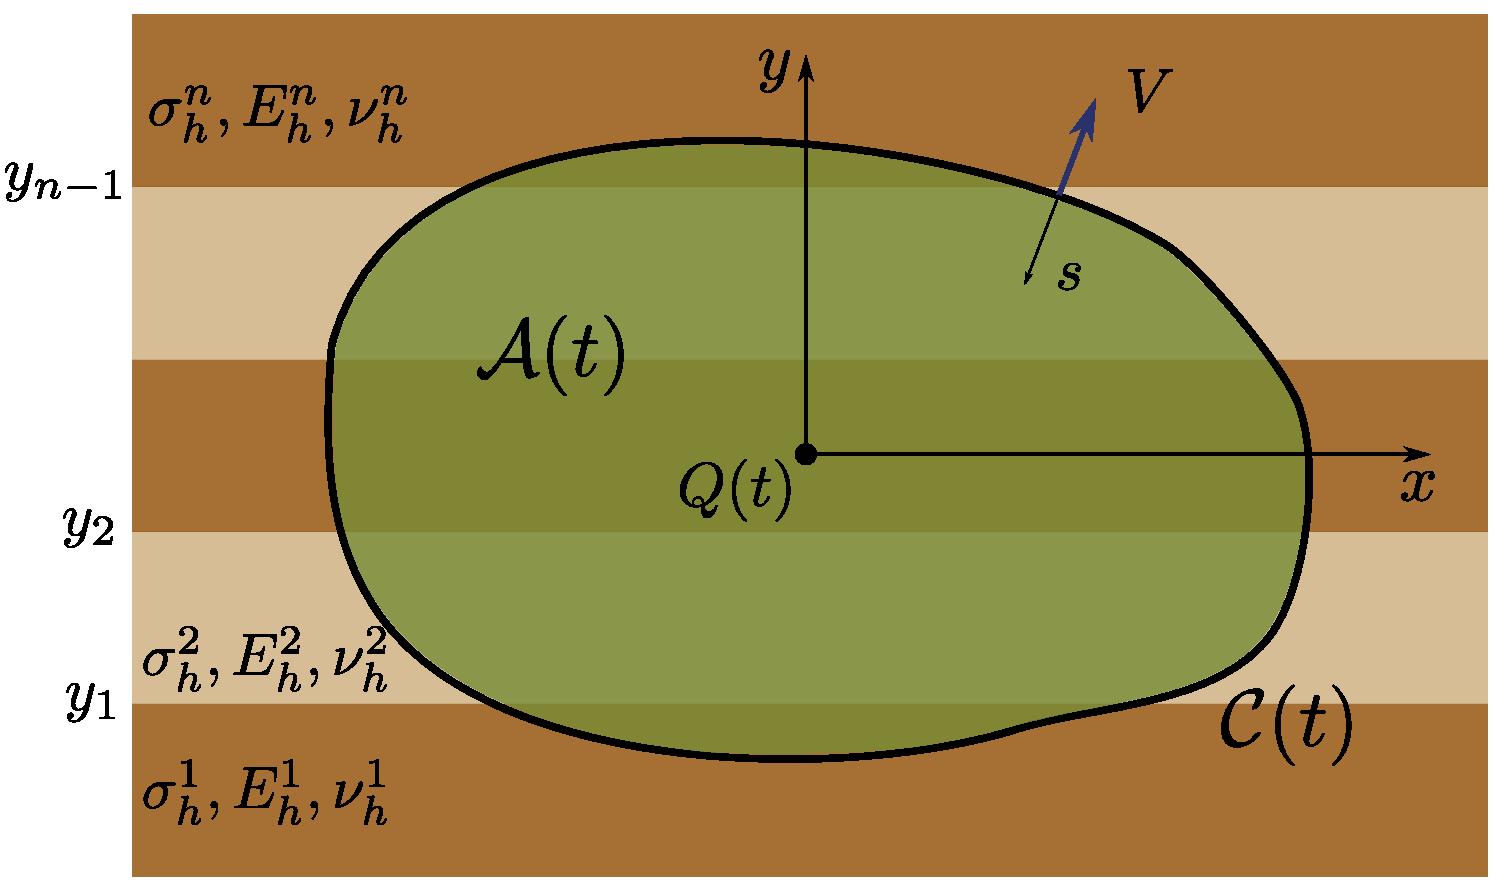
\includegraphics[width=0.8\textwidth]{fracture_scheme.pdf}
\end{frame}

\subsection{Определяющие уравнения}
\begin{frame}
    \frametitle{Модель плоской трещины ГРП}
    Уравнение Рейнольдса (закон сохранения массы)
    \begin{equation}
        \label{eq:reynolds_equation}
        \pd{w}{t} - \text{div} \left(\frac{w^3}{12\mu} \bigtriangledown \!p \right) + \frac{2C_L}{\sqrt{t-t_0(x,\, y)}}  = Q(t) \delta(x,\,y),
    \end{equation}

    Уравнение упругости
    \begin{equation}
        \label{eq:elasticity_equation}
        p(x,y,t) = \sigma_h(y) + \int\limits_{\mathcal{A}(t)} G(x,y;x',y')w(x',y',t) \dif x' \dif y',
    \end{equation}

    Граничные условия на движущемся фронте
    \begin{minipage}{0.49\textwidth}
        \begin{equation*}
            \lim_{s \to 0} \frac{w(s)}{s^{1/2}}=\frac{K'}{E'},
        \end{equation*}
    \end{minipage}
    \hfill
    \begin{minipage}{0.5\textwidth}
        \begin{equation}
            \lim_{s \to 0} \frac{w^3}{12\mu} \pd{p}{s}=0.
        \end{equation}
    \end{minipage}
\end{frame}

\begin{frame}
    \frametitle{Постановка задачи}
    В институте гидродинамики им. М. А. Лаврентьева СО РАН ранее был реализован симулятор ГРП Planar3D ILSA в предположении
    \begin{equation}
        \label{eq: heterogeneous_elasticity_equation}
        p(x,y,t) = \sigma_h(y) - \frac{E'}{8\pi}\int\limits_{\mathcal{A}(t)} \frac{w(x',y',t)}{[(x\!-\!x')^2+(y\!-\!y')^2]^{3/2}} \dif x' \dif y'.
    \end{equation}

    Целью данной работы является 
    \begin{itemize}
        \item реализация метода построения численной матрицы жесткости для слоистой среды с неоднородностью по модулям упругости и внедрение его в модель Planar3D ILSA,
        \item анализ влияния неоднородности модулей упругости на геометрию трещины ГРП,
        \item сравнение влияния неоднородности сжимающих напряжений и модулей упругости слоев на геометрию финальной трещины ГРП,
        \item анализ влияния тонких жестких пропластков на рост и раскрытие трещины ГРП.
    \end{itemize}
\end{frame}

\section{Численное построение матрицы упругости}
\begin{frame}
    \frametitle{Численное построение матрицы жесткости}
    Метод численного построения был предложен Энтони Пирсом \footfullcite{Peirce2001TheSF}.
    Для каждого слоя записываем уравнение равновесия для упругой изотропной среды
    \begin{equation}
        \label{eq:equilibrium}
        \sigma_{ij,j} + f_i = 0,
    \end{equation}
    закон Гука
    \begin{equation}		
        \sigma_{ij} = \lambda e_{kk}\delta_{ij} + 2G e_{ij}.
        \label{eq:hooke_law}
    \end{equation}
    На границе раздела слоев выполняется условие непрерывности компонент вектора смещений и нормальной нагрузки. Тогда ядро в интегральном соотношении~\eqref{eq:elasticity_equation}
    \begin{equation}
        \begin{split}
            G(x,y,x',y') & = \sigma_{zz}(x,y), \\
            \left[u_{z} \right]_{(x',y')} & = \left.u_{z-0} - u_{z+0}\right|_{(x',y')} = 1.
        \end{split}
    \end{equation}
\end{frame}

\begin{frame}
    \frametitle{Введение псевдо-границы}
    \begin{minipage}[t]{0.47\linewidth}
        \footnotesize{Условие точечного разрыва смещений}
        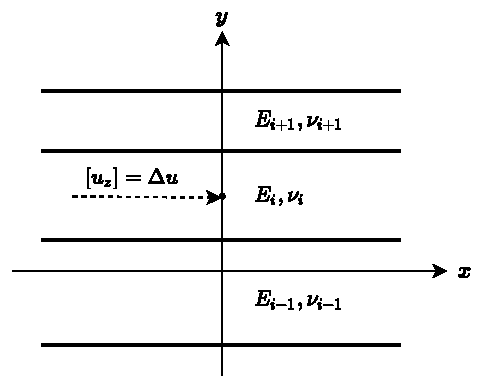
\includegraphics[width=\linewidth]{DD_point.pdf}
    \end{minipage}
    \hfill
    \begin{minipage}[t]{0.47\linewidth}
        \footnotesize{Введение дополнительной границы}
        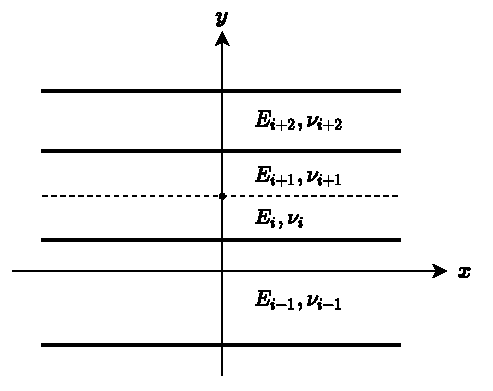
\includegraphics[width=\linewidth]{DD_point2.pdf}
    \end{minipage}
    Тогда $u_{z-0} - u_{z+0} = \Delta u$ может быть представлена в виде скачка смещений и напряжений на псевдо-границе $\left[ T \right] = T(y-0) - T(y+0)$, где $T = \left[\sigma_{yy} , \quad \sigma_{xy} , \quad \sigma_{yz} , \quad u_{y} , \quad u_{x} , \quad u_{z}\right]^T$.
\end{frame}

\begin{frame}
    \frametitle{Постановка в Фурье-образе}
    Записываем определяющие уравнения в виде
    \begin{equation}
        \label{eq:separate}
        \partial_{y} T = \mathbb{A}T,
    \end{equation}

    и применяя двумерное преобразование Фурье по координатам $x$ и $z$, получим
    \begin{equation}
        \label{eq:FT_system}
        \partial_y \hat{T} = \hat{\mathbb{A}} \hat{T}.
    \end{equation}
    Система \eqref{eq:FT_system} является ОДУ и решение зависит от 6 спектральных коэффициентов $A(m,n)$ (константы интегрирования)
    \begin{equation}
        \label{eq:fourier_solution}
        \hat{T} = \mathbb{Z}A.
    \end{equation}
    Связь между спектральными коэффициентами и значениями смещений и напряжений на границе слоя
    \begin{equation}
        A(m,n) = \mathbb{Z}^{-1}\hat{T}(y=y_i).
    \end{equation}
\end{frame}

\begin{frame}
    \frametitle{Связанная система уравнений для граничных значений}
    Из этих соотношений можно составить уравнения для определения компонент вектора смещения и напряжений на границе раздела слоев
    \begin{equation}
        \label{eq:coupled-system}
        \textbf{A}^i \hat{T}_{y=y_{i-1}} +
        \textbf{C}^i \hat{T}_{y=y_{i}} + 
        \textbf{B}^i \hat{T}_{y=y_{i+1}}
        = \textbf{D}^i,
    \end{equation}
    Ядро $G(x,y;x',y')$ интегрального соотношения~\eqref{eq:elasticity_equation} для слоистой среды
    \begin{equation}
        G(x,y;x',y') = G_\text{hom}(x,y;x',y') + G'(x,y;x',y'),
    \end{equation} 
    где
    \begin{equation}
        \begin{split}
            G_\text{hom}(x,y;x',y') & = - \frac{E'(y)}{8\pi [(x\!-\!x')^2+(y\!-\!y')^2]^{3/2}},\\
            G'(x,y;x',y') & = \Delta \sigma_{zz}(x,y),\\
            \left[u_{z} \right]_{(x',y')} & = \left.u_{z-0} - u_{z+0}\right|_{(x',y')} = 1.
        \end{split}
    \end{equation}
    где $\sigma_{zz}(x,y)$ находится из $\hat{\sigma}_{zz}(m,n)$ путем применения обратного дискретного преобразования Фурье.
\end{frame}

\begin{frame}
    \centering
    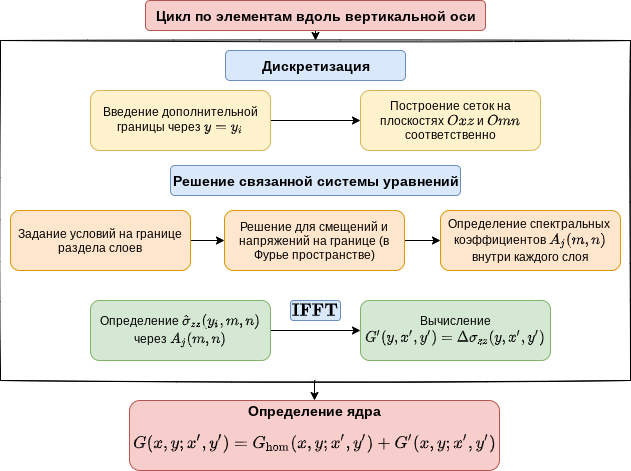
\includegraphics[width=0.9\textwidth]{scheme-layered.png}
\end{frame}


\section{Верификация и численные расчеты}

\begin{frame}[t]
    \frametitle{Верификация}
    \begin{columns}
        \begin{column}{0.4\textwidth}
            Численная сходимость метода
            \begin{enumerate}
                \item $E_{max} = \frac{||\mathbf{w}_h - \mathbf{w}||_{L_\infty}}{||\mathbf{w}||_{L_\infty}}$
                \item $E_2 = \frac{||\mathbf{w}_h - \mathbf{w}||_{L_2}}{||\mathbf{w}||_{L_2}}$
            \end{enumerate}
        \end{column}
        \begin{column}{0.55\textwidth}
            \centering
            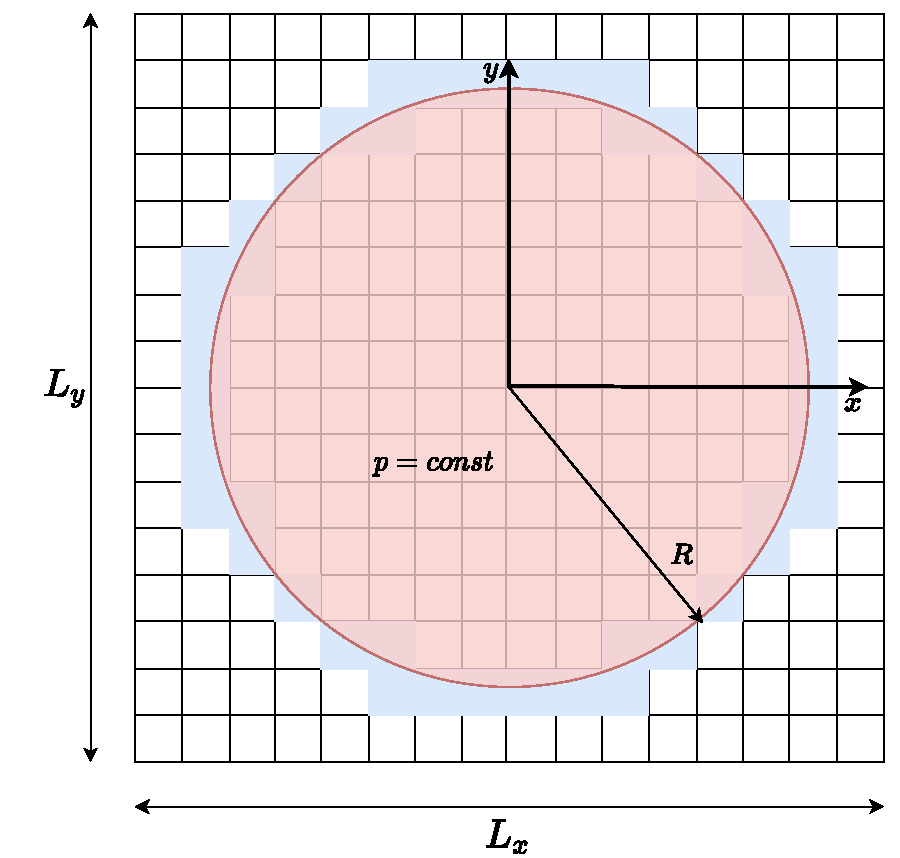
\includegraphics[width=\textwidth]{radial_fracture.pdf}
        \end{column}
    \end{columns}
\end{frame}

\begin{frame}
    \centering
    \begin{figure}
        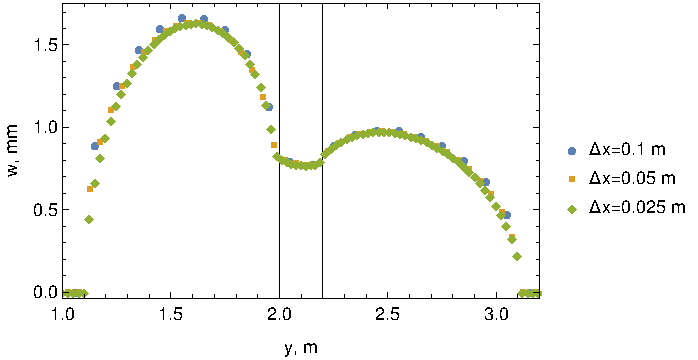
\includegraphics[width=0.7\textwidth]{static_accuracy.pdf}
        \caption{\footnotesize{Трехслойная среда, модуль Юнга и коэффициент Пуассона в слоях равны 1, 10, 2 GPa и 0.1, 0.4, 0.2 соответственно.}}
    \end{figure}

    \begin{tabular}{|c|c|c|}
        \hline
        $\Delta x, \text{м}$ & $E_{max}$ & $E_2$ \\
        \hline
        0.1                     & 0.129     & 0.059 \\
        \hline
        0.05                    & 0.096     & 0.028 \\
        \hline
        0.025 & --- & --- \\
        \hline
    \end{tabular}
\end{frame}

\begin{frame}
    \frametitle{Радиальная трещина, $E_\text{b} = E_\text{m} = E_\text{t} = 10$~GPa, $\nu_\text{b} = \nu_\text{m} = \nu_\text{t} = 0.22$}
    \begin{minipage}[t]{0.4\linewidth}
        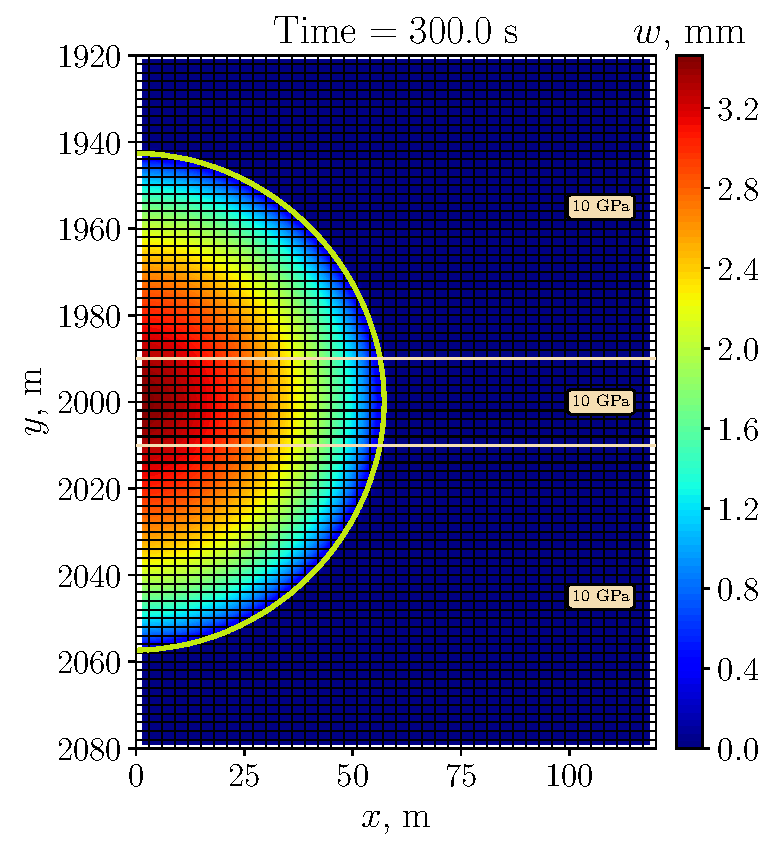
\includegraphics[width=\linewidth]{Homogeneous/Figures/1/width_29.pdf}
    \end{minipage}
    \hfill
    \begin{minipage}[t]{0.57\linewidth}
        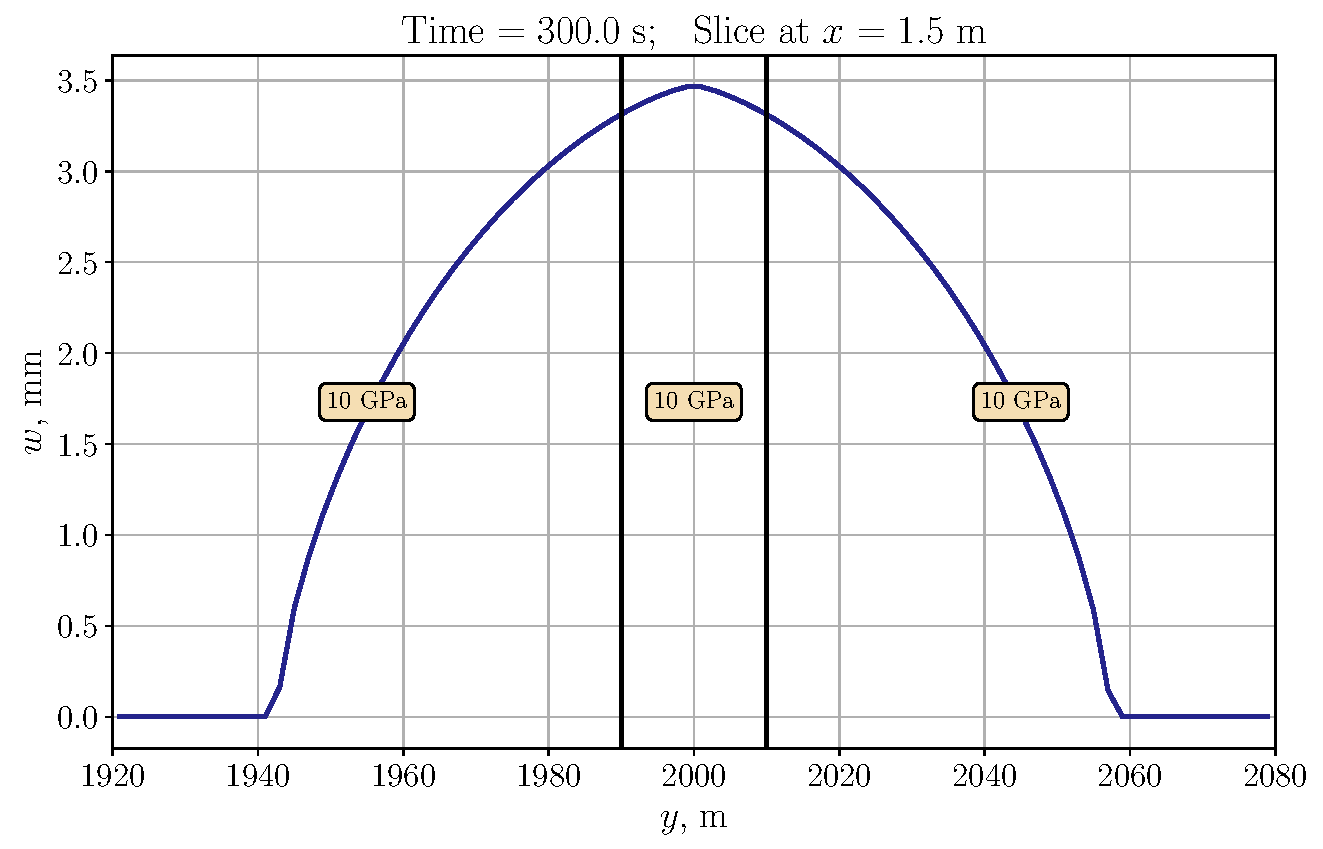
\includegraphics[width=\linewidth]{Homogeneous/Figures/1/w_y_29.pdf}
    \end{minipage}
\end{frame}

\begin{frame}
    \frametitle{Пласт с жестким нижним слоем, $E_\text{b} = 50$~GPa, $E_\text{m} = E_\text{t} = 10$~GPa, $\nu_\text{b} = \nu_\text{m} = \nu_\text{t} = 0.22$}
    \begin{minipage}[t]{0.4\linewidth}
        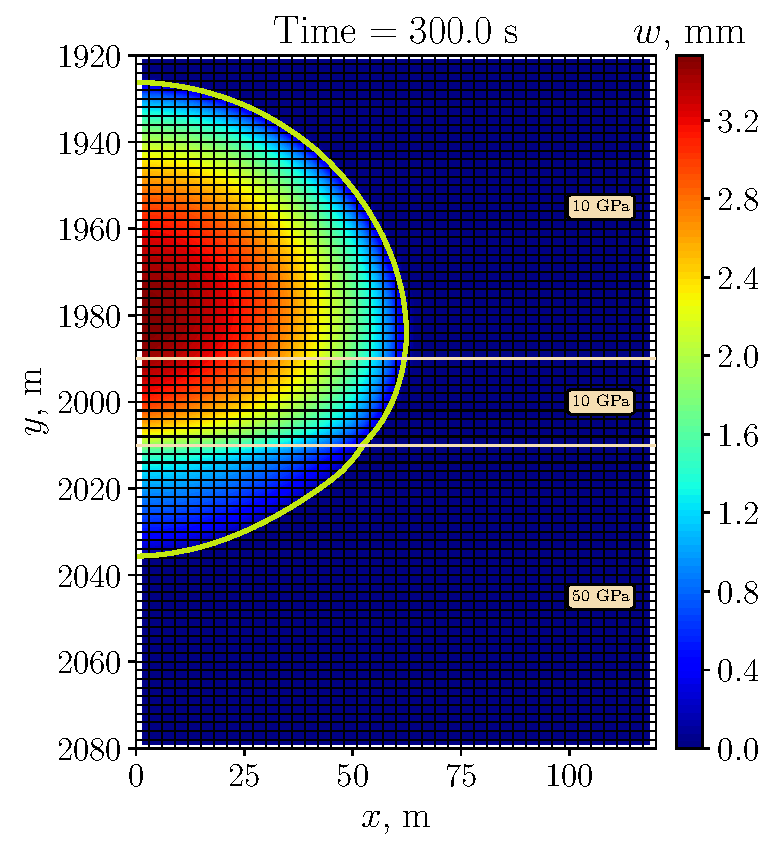
\includegraphics[width=\linewidth]{Heterogeneous/Figures/1/width_29.pdf}
    \end{minipage}
    \hfill
    \begin{minipage}[t]{0.57\linewidth}
        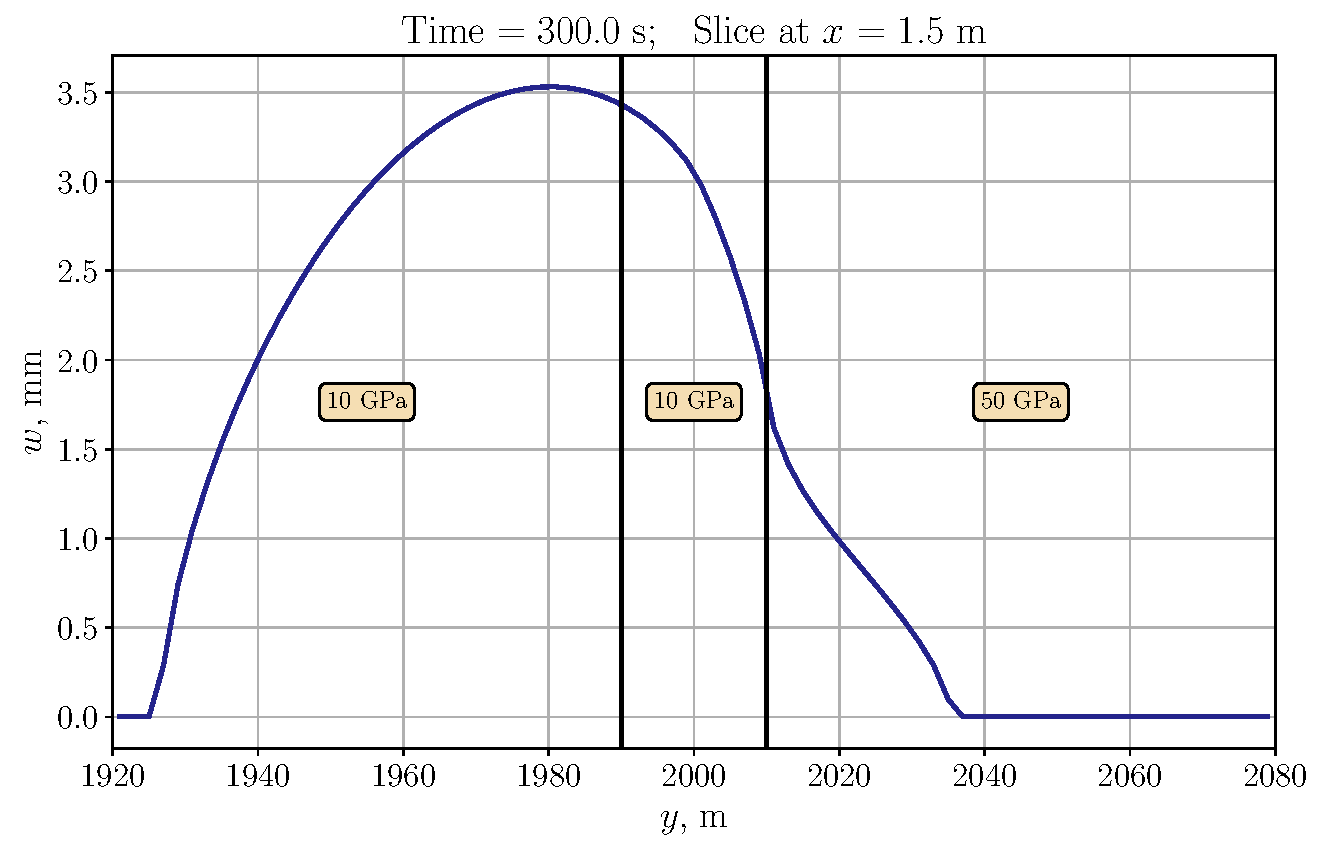
\includegraphics[width=\linewidth]{Heterogeneous/Figures/1/w_y_29.pdf}
    \end{minipage}
\end{frame}

\begin{frame}
    \frametitle{Пласт с сильной неоднородностью, $E_\text{b} = 100$~GPa, $E_\text{m} = E_\text{t} = 10$~GPa, $\nu_\text{b} = \nu_\text{m} = \nu_\text{t} = 0.22$}
    \begin{minipage}[t]{0.4\linewidth}
        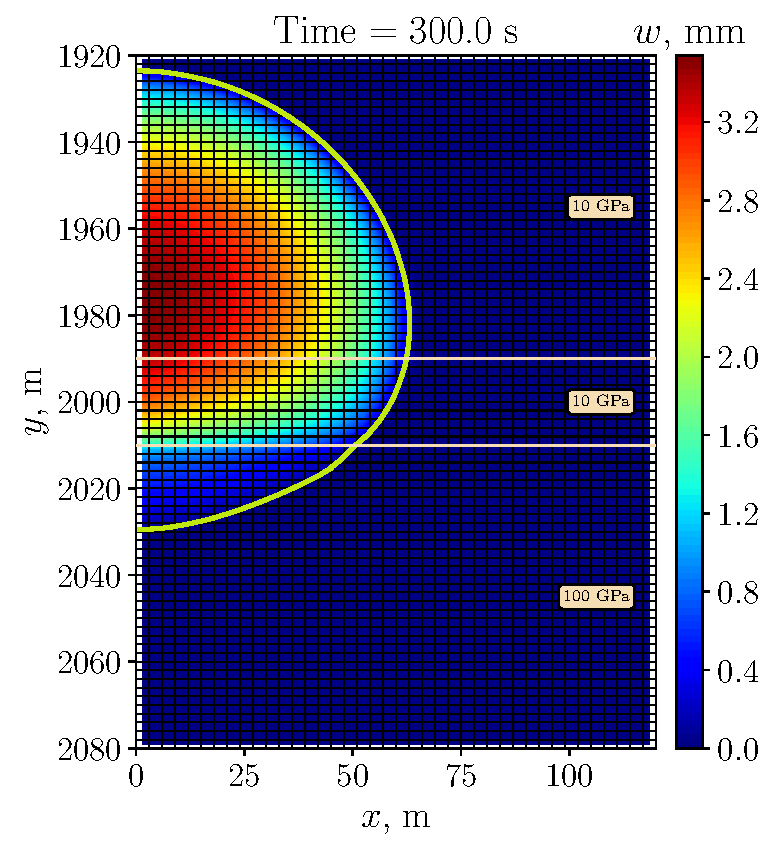
\includegraphics[width=\linewidth]{Heterogeneous/Figures/2/width_29.pdf}
    \end{minipage}
    \hfill
    \begin{minipage}[t]{0.57\linewidth}
        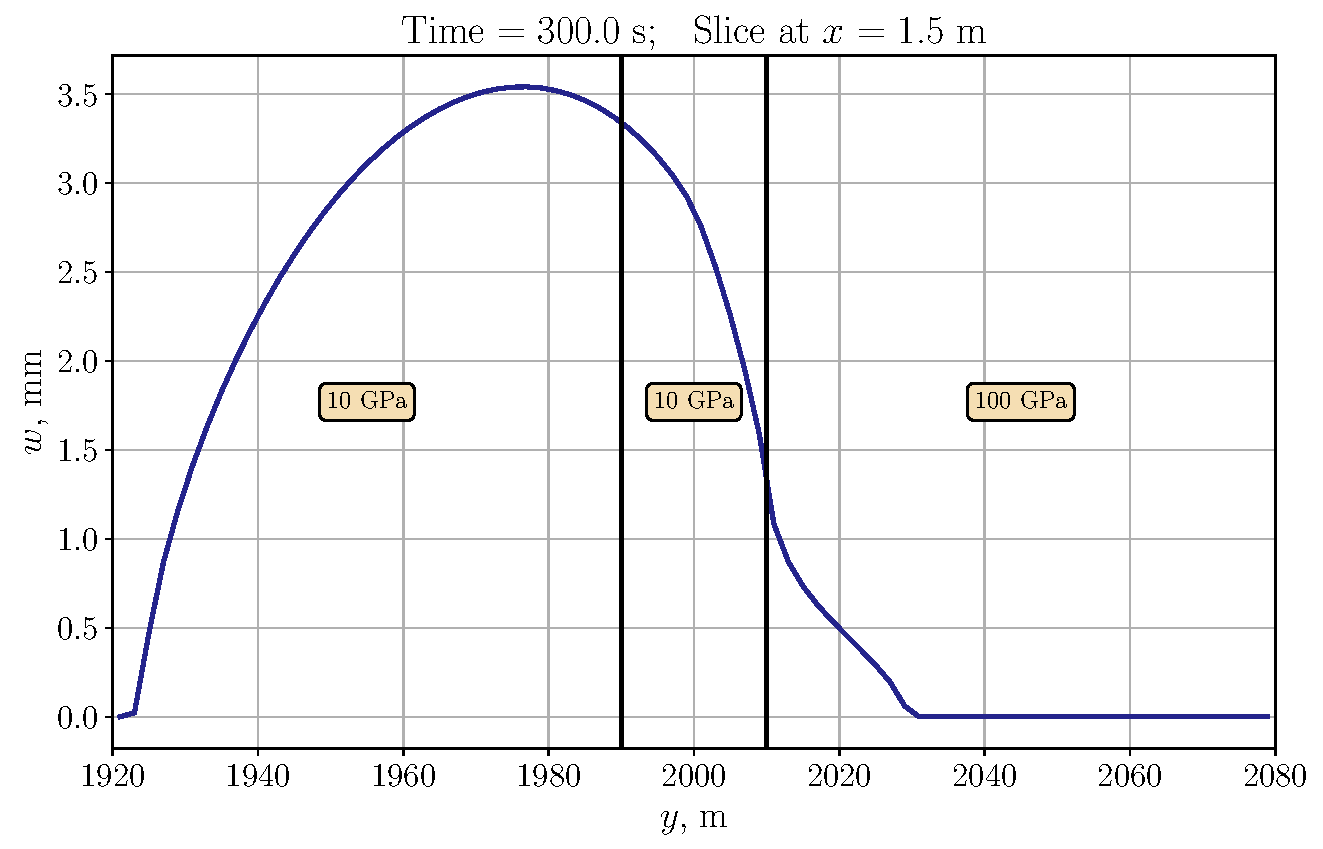
\includegraphics[width=\linewidth]{Heterogeneous/Figures/2/w_y_29.pdf}
    \end{minipage}
\end{frame}

\begin{frame}
    \frametitle{Пласт с сильной неоднородностью, $E_\text{m} = 10$~GPa, $E_\text{b} = E_\text{t} = 100$~GPa, $\nu_\text{b} = \nu_\text{m} = \nu_\text{t} = 0.22$}
    \begin{minipage}[t]{0.4\linewidth}
        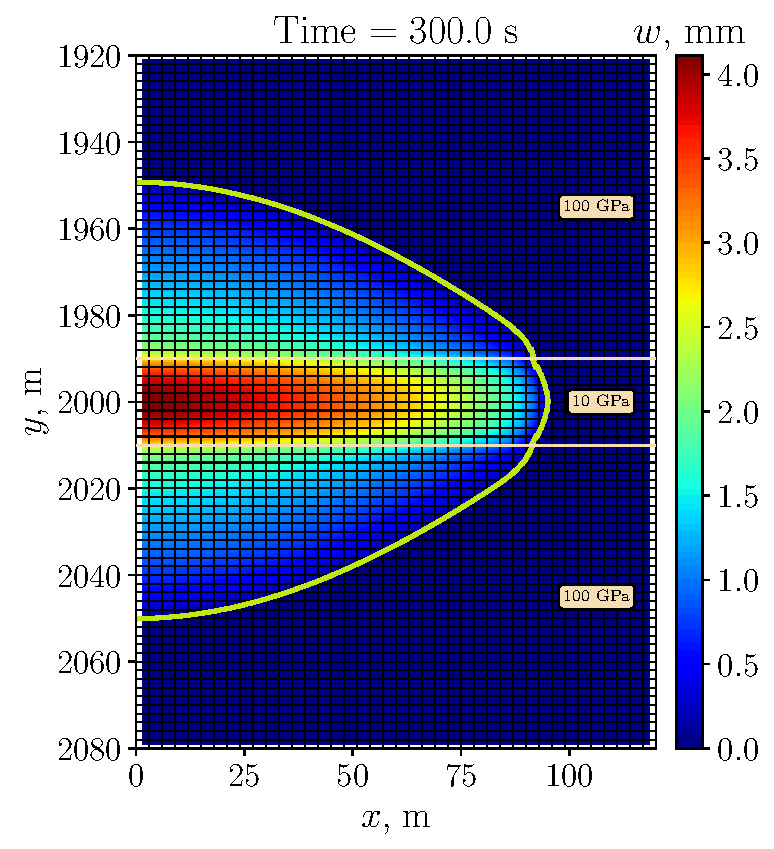
\includegraphics[width=\linewidth]{Heterogeneous/Figures/3_3/width_29.pdf}
    \end{minipage}
    \hfill
    \begin{minipage}[t]{0.57\linewidth}
        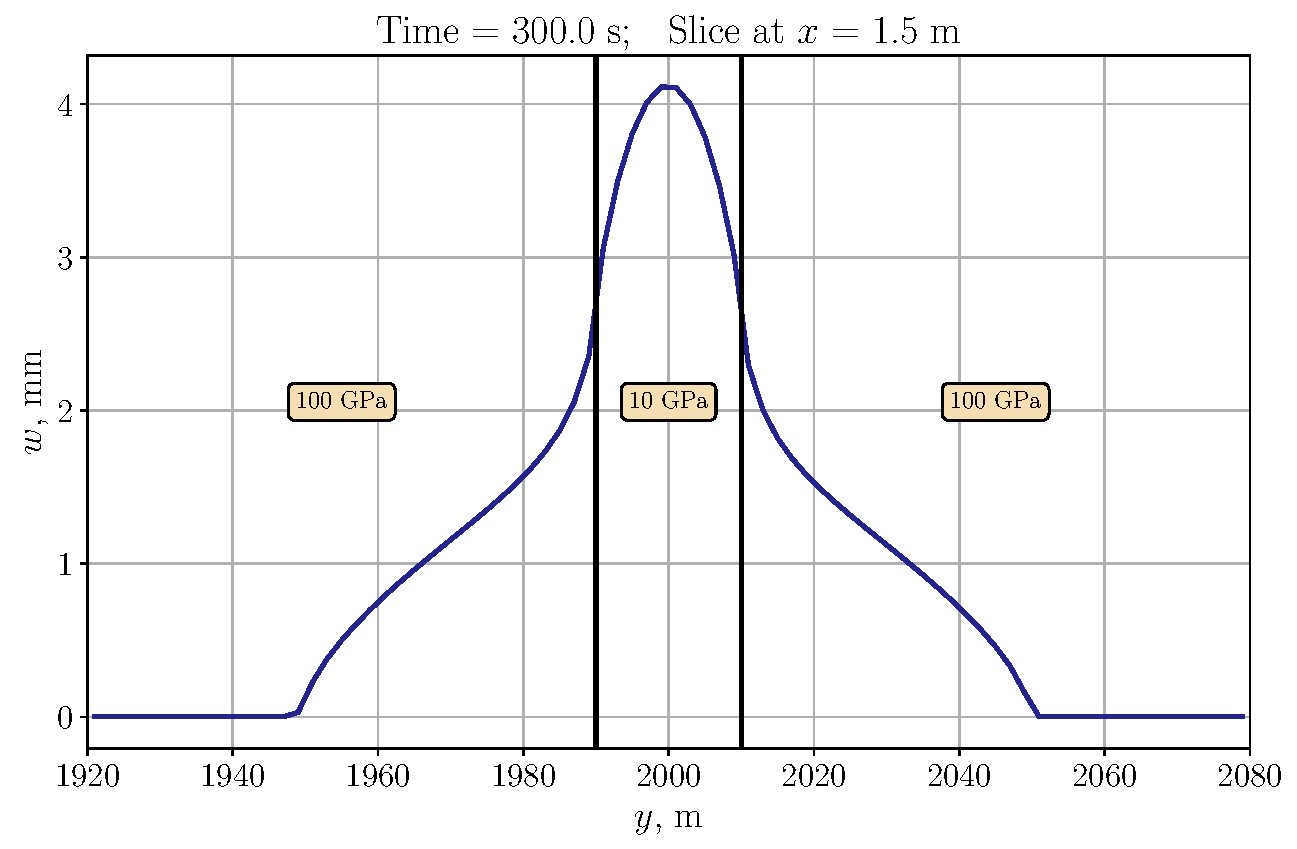
\includegraphics[width=\linewidth]{Heterogeneous/Figures/3_3/w_y_29.pdf}
    \end{minipage}
\end{frame}

\begin{frame}
    \frametitle{$E_\text{b} = 20$~GPa, $E_\text{m} = E_\text{t} = 10$~GPa, $\nu_\text{b} = \nu_\text{m} = \nu_\text{t} = 0.22$, $\sigma_{h,\text{b}} = 30$~MPa, $\sigma_{h,\text{m}} = \sigma_{h,\text{t}} = 30.5$~MPa}
    \begin{minipage}[t]{0.4\linewidth}
        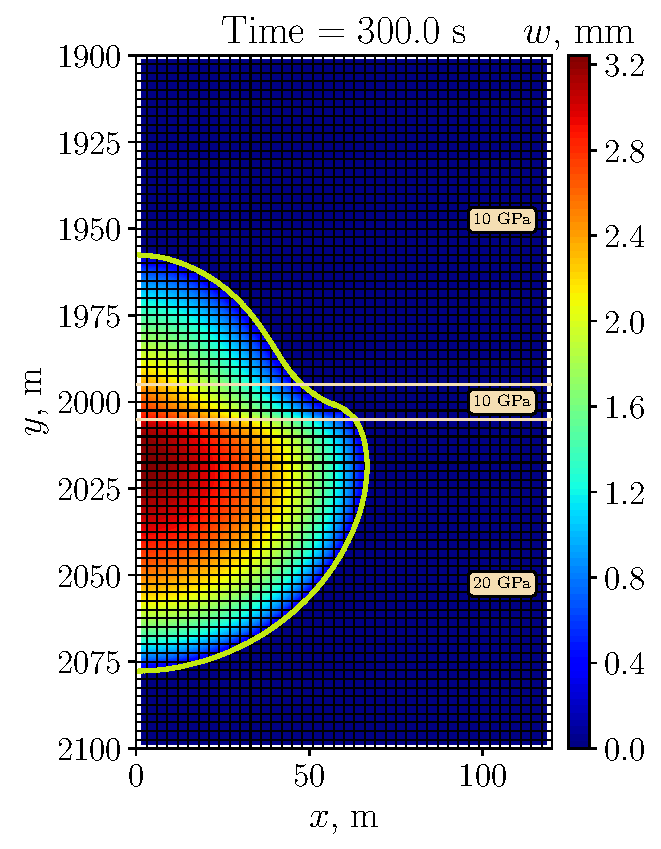
\includegraphics[width=\linewidth]{Heterogeneous/Figures/3/width_29.pdf}
    \end{minipage}
    \hfill
    \begin{minipage}[t]{0.57\linewidth}
        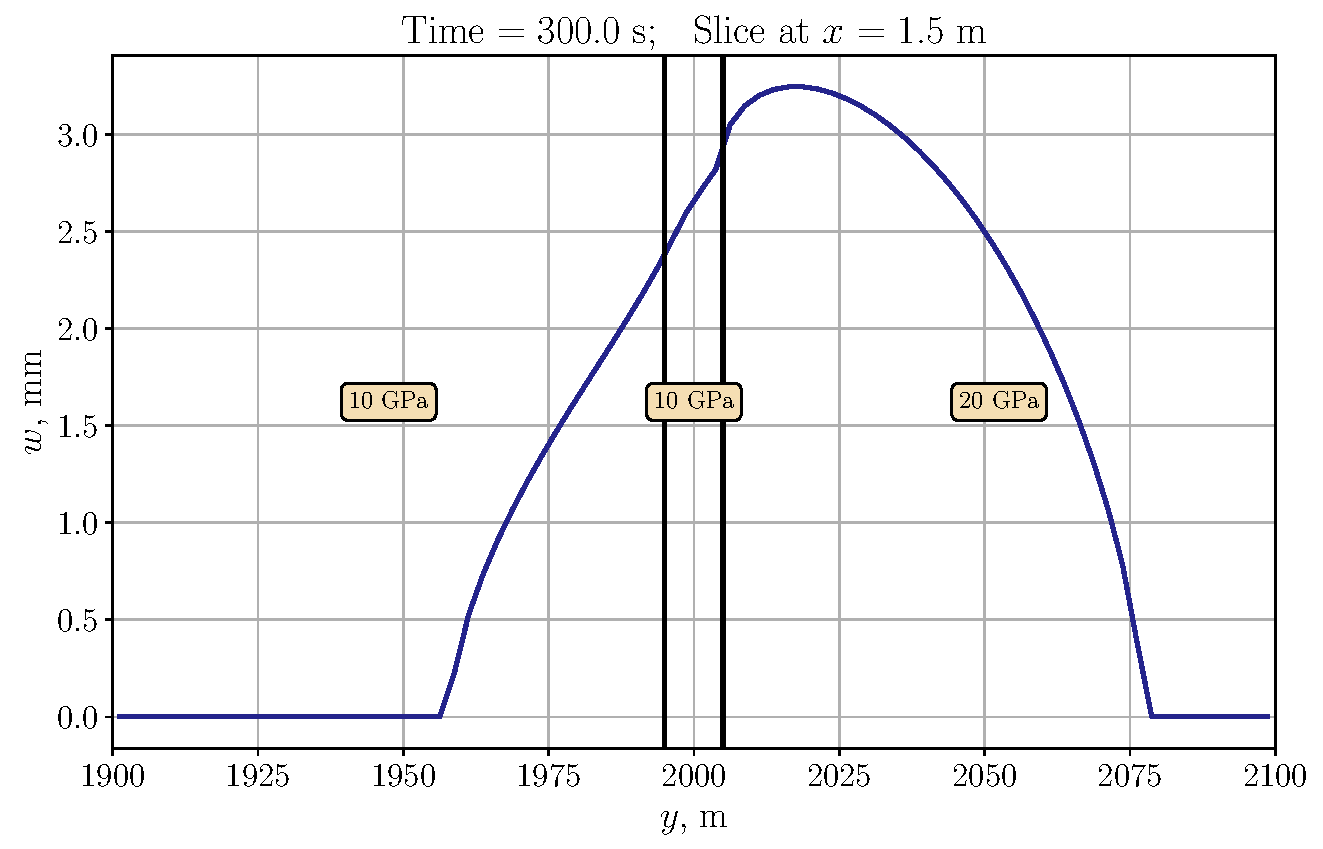
\includegraphics[width=\linewidth]{Heterogeneous/Figures/3/w_y_29.pdf}
    \end{minipage}
\end{frame}

\begin{frame}
    \frametitle{$E_\text{b} = 40$~GPa, $E_\text{m} = E_\text{t} = 10$~GPa, $\nu_\text{b} = \nu_\text{m} = \nu_\text{t} = 0.22$, $\sigma_{h,\text{b}} = 30$~MPa, $\sigma_{h,\text{m}} = \sigma_{h,\text{t}} = 30.5$~MPa}
    \begin{minipage}[t]{0.4\linewidth}
        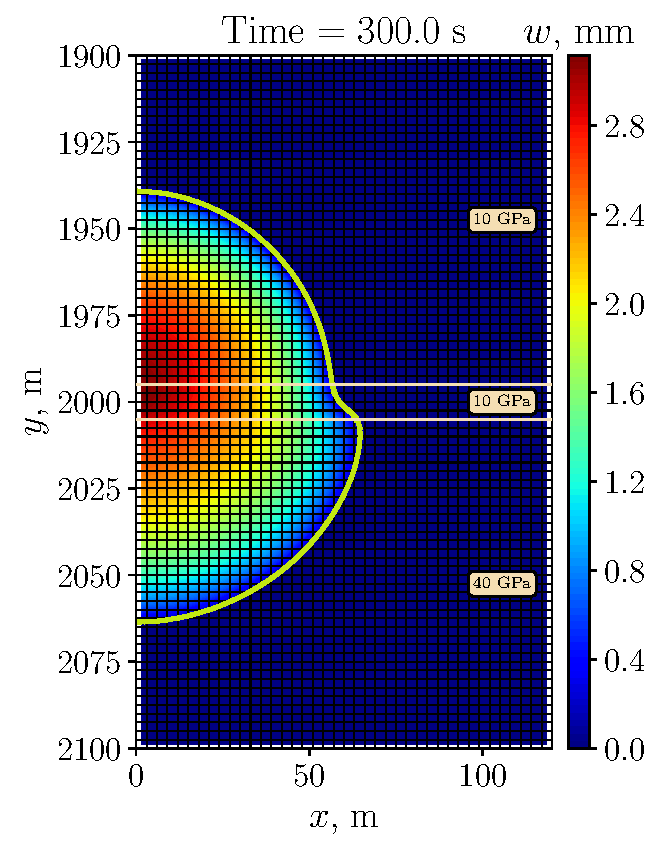
\includegraphics[width=\linewidth]{Heterogeneous/Figures/3_2/width_29.pdf}
    \end{minipage}
    \hfill
    \begin{minipage}[t]{0.57\linewidth}
        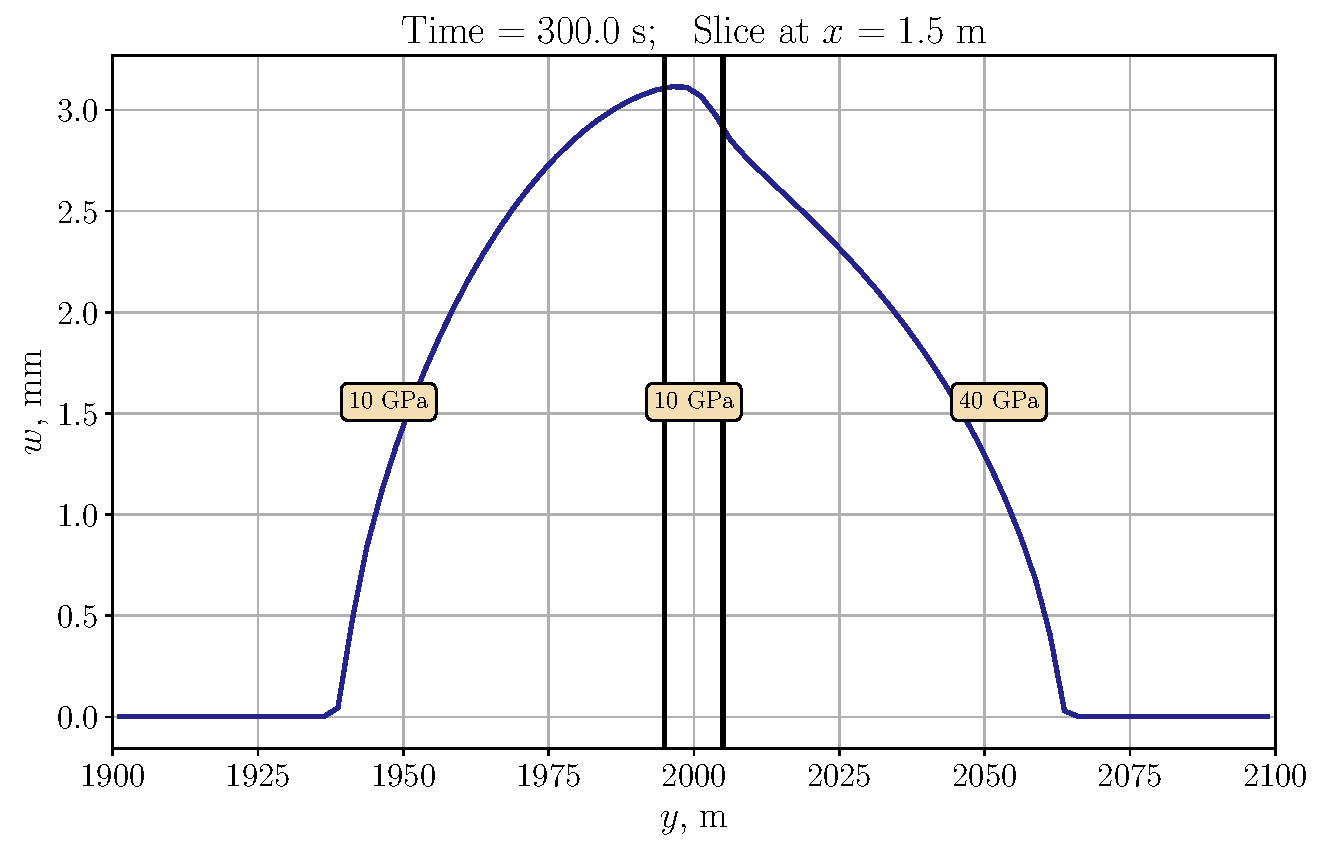
\includegraphics[width=\linewidth]{Heterogeneous/Figures/3_2/w_y_29.pdf}
    \end{minipage}
\end{frame}

\begin{frame}
    \frametitle{Пласт с включением тонкого слоя, $d=10$~м. , $k=\frac{E_d}{E}=5$}
    \begin{minipage}[t]{0.4\linewidth}
        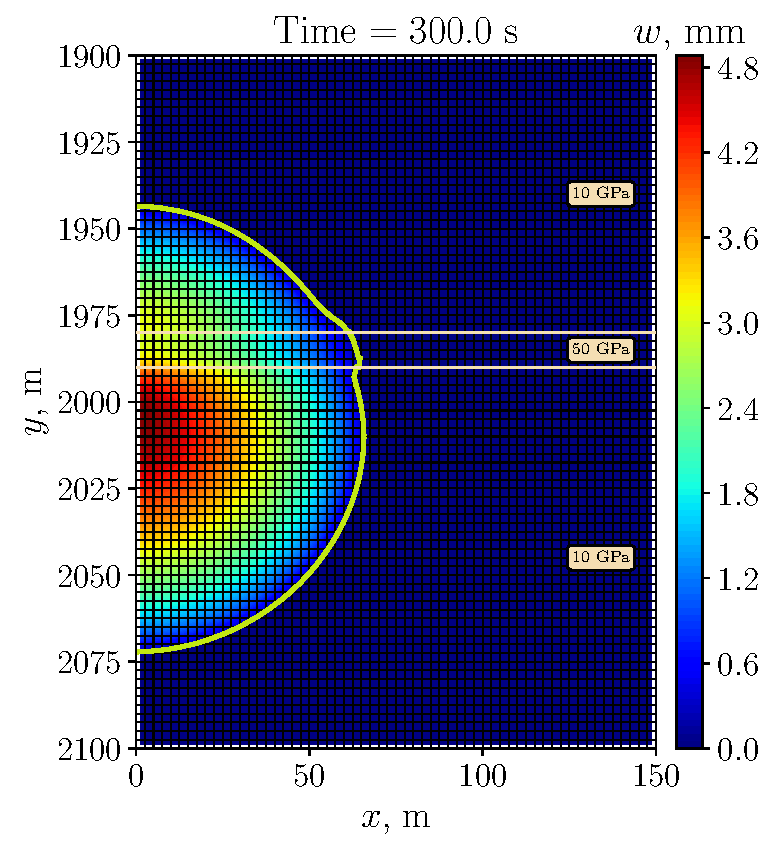
\includegraphics[width=\linewidth]{Heterogeneous/Figures/4/width_29.pdf}
    \end{minipage}
    \hfill
    \begin{minipage}[t]{0.57\linewidth}
        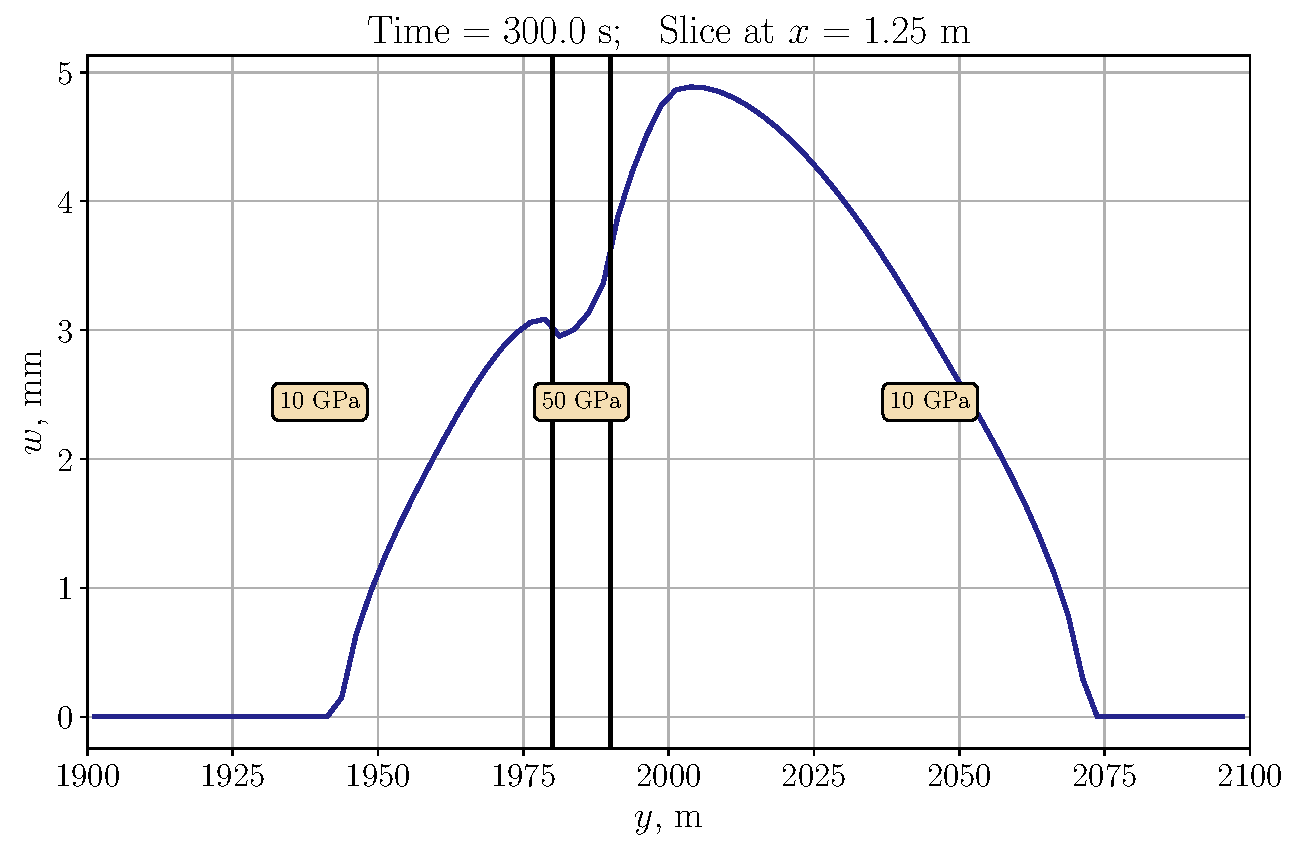
\includegraphics[width=\linewidth]{Heterogeneous/Figures/4/w_y_29.pdf}
    \end{minipage}
\end{frame}

\begin{frame}
    \frametitle{Пласт с включением двух тонких пропластков, $d=10$~м. , $k=\frac{E_d}{E}=5$}
    \begin{minipage}[t]{0.4\linewidth}
        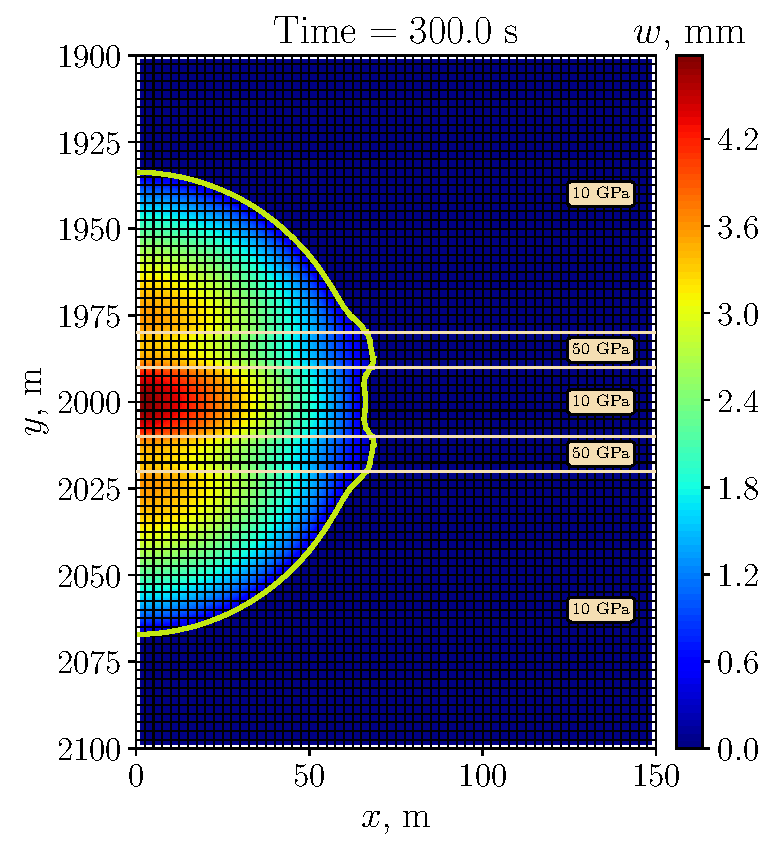
\includegraphics[width=\linewidth]{Heterogeneous/Figures/5/width_29.pdf}
    \end{minipage}
    \hfill
    \begin{minipage}[t]{0.57\linewidth}
        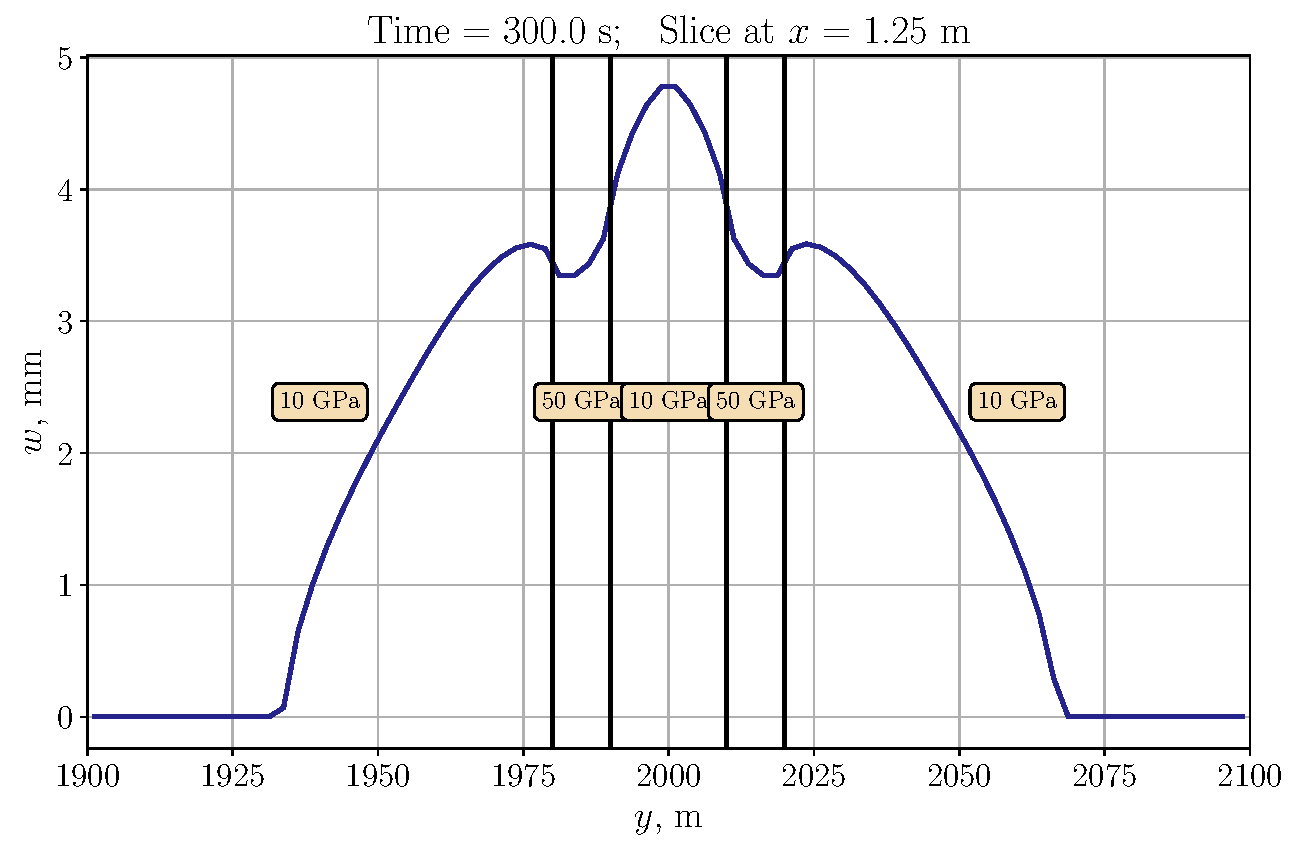
\includegraphics[width=\linewidth]{Heterogeneous/Figures/5/w_y_29.pdf}
    \end{minipage}
\end{frame}       % Настройки заглавной странице
\section{Заключение}
\begin{frame}
    \frametitle{Заключение}
    \textbf{Основные результаты работы} заключаются в следующем:
    \begin{itemize}
        \item Реализован алгоритм построения численной матрицы упругости для метода разрывных смещений в случае неоднородных по модулю упругости слоев на языке программирования~C++.
        \item Выполнено встраивание данного алгоритма в модель раскрытия трещины гидроразрыва пласта Planar3d ILSA.
        \item Проведена верификация метода путем сравнения с известными литературными данными и точными решениями.
        \item Проведен анализ влияния учета слоистой структуры пласта на конечную геометрию трещины.
        \item Показано, что тонкие жесткие пропластки не существенно ограничивают рост трещины в вертикальном направлении, однако влияют на раскрытие трещины в них, что может сильно сказаться на распространение проппанта и конечной геометрии трещины ГРП. 
    \end{itemize}
\end{frame}

% \begin{frame} % публикации на одной странице
% % \begin{frame}[t,allowframebreaks] % публикации на нескольких страницах
%     \frametitle{Основные публикации}
%     \nocite{vakbib1}%
%     \nocite{vakbib2}%
%     %
%     %% authorwos
%     \nocite{wosbib1}%
%     %
%     %% authorscopus
%     \nocite{scbib1}%
%     %
%     %% authorconf
%     \nocite{confbib1}%
%     \nocite{confbib2}%
%     %
%     %% authorother
%     \nocite{bib1}%
%     \nocite{bib2}%
%     \ifnumequal{\value{bibliosel}}{0}{
%         \insertbiblioauthor
%     }{
%         \printbibliography%
%     }
% \end{frame}
    % Последние слайды презентации
\appendix
\begin{frame}
    \frametitle{Дифференциальный оператор}
    \begin{equation*}
        \mathbb{A} = 
        \left[\begin{array}{cccccc}
            0                      & -\partial_x & -\partial_z & 0 & 0 & 0 \\
            -\frac{b}{a}\partial_x & 0           & 0 & 0 & \frac{b^2-a^2}{a}\partial_{xx} - \frac{f}{2}\partial_{zz} & \left( \frac{b^2-ab}{a} - \frac{f}{2} \right) \partial_{xz} \\
            -\frac{b}{a}\partial_z & 0           & 0 & 0 & \left( \frac{b^2-ab}{a} - \frac{f}{2} \right) \partial_{xz} & \frac{b^2-a^2}{a}\partial_{zz} - \frac{f}{2}\partial_{xx} \\
            \frac{1}{a}            & 0           & 0 & 0 & -\frac{b}{a}\partial_x & -\frac{b}{a}\partial_z \\
            0                      & \frac{2}{f} & 0 & -\partial_x & 0 & 0 \\
            0                      & 0           & \frac{2}{f} & -\partial_z & 0 & 0 
        \end{array}\right],
    \end{equation*}
    
    где используются константы
    \begin{align*}
        a   & = \lambda + 2G,                          & b   & = \lambda,                &     f & = 2G, \\
        l_2 & = \frac{\lambda + 3G}{\lambda + G},      & l_4 & = \frac{2G^2}{\lambda+G}, &   l_5 & = \frac{2G(\lambda + 2G)}{\lambda + G}, \\
        l_6 & = \frac{2G(2\lambda + 2G)}{\lambda + G}, & l_7 & = \frac{2\lambda G}{\lambda+G}
    \end{align*}
\end{frame}

\begin{frame}
    \frametitle{Обозначения}
    \begin{equation}
        \label{eq:FT_special_variables}
        \begin{split}
            \hat{u}_s & = -i \frac{(m\hat{u}_x + n\hat{u}_z)}{k}, \\
            \hat{u}_t & = -i \frac{(n\hat{u}_x - m\hat{u}_z)}{k}, \\
            \hat{\tau}_s & = -i \frac{(m\hat{\sigma}_{xy} + n\hat{\sigma}_{yz})}{k}, \\
            \hat{\tau}_t & = -i \frac{(n\hat{\sigma}_{xy} - m\hat{\sigma}_{yz})}{k}. \\
        \end{split} 
    \end{equation}

    \begin{equation}
        \begin{split}
        Z_s & = 
        \left[
        \begin{array}{cccc}
            -fe^{-ky} & (l_4-fky)e^{-ky} & fe^{ky} & (l_4+fky)e^{ky} \\
            -fe^{-ky} & (l_5-fky)e^{-ky} & -fe^{ky} & -(l_5+fky)e^{ky} \\
            e^{-ky} & kye^{-ky} & e^{ky} & kye^{ky} \\
            e^{-ky} & (ky-l_2)e^{-ky} & -e^{ky} & -(ky+l_2)e^{ky} \\
        \end{array}
        \right],
        \\
        Z_t & = 
        \left[
        \begin{array}{cc}
            -\frac{f}{2}e^{-ky} & \frac{f}{2}e^{ky} \\
            e^{-ky} & e^{ky}
        \end{array}
        \right].
        \end{split}
    \end{equation}
\end{frame}

\begin{frame}
    \frametitle{Условие скачка смещений и напряжений на границе раздела псевдослоя}
    \begin{equation*}
        \left[ \hat{T} \right] = 
        \left[ \begin{array}{c} 
            0 \\ \frac{\Delta u(b^2 - a^2)}{a} \\ \frac{\Delta ub}{a} \\ 0 \\ 0 \\ 0 
        \end{array} \right]
        +
        \frac{m^2}{m^2+n^2} \left[ \begin{array}{c} 
            0 \\ \Delta u(a-b) \\ 0 \\ 0 \\ 0 \\ 0 
        \end{array} \right]
        +
        \frac{mn}{m^2+n^2} \left[ \begin{array}{c} 
            0 \\ 0 \\ 0 \\ 0 \\ \Delta u(a-b) \\ 0 
        \end{array} \right].
    \end{equation*}
\end{frame}

\begin{frame}
    \frametitle{t-система связанных уравнений}
    Коэффициенты в t-системе \eqref{eq:coupled_t-system} имеют вид
    \begin{equation*}
        \begin{split}
            A^{i}_t &= \frac{2}{f^{i}}\text{cosech}(kd^{i}),\\
            B^{i}_t &= \frac{2}{f^{i+1}}\text{cosech}(kd^{i+1}),\\
            C^{i}_t &= -\frac{2}{f^{i+1}}\coth(kd^{i+1}) - \frac{2}{f^{i}}\coth(kd^{i}),\\
            D^{i}_t &= \Delta \hat{u}^{i}_{t} + \frac{2}{f^{i+1}}\coth(kd^{i+1})\Delta\hat{\tau}_{t}^{i} 
            - \frac{2}{f^{i}}\text{cosech}(kd^{i})\Delta\hat{\tau}_{t}^{i-1},
        \end{split}
    \end{equation*}
    \begin{equation*}
        \hat{u}^{i}_{t} = \frac{2}{f^{i}}\coth(kd^{i})\hat{\tau}^{i}_{t} - \frac{2}{f^{i}}\text{cosech}(kd^{i}) (\hat{\tau}^{i-1}_{t} + \Delta\hat{\tau}^{i-1}_{t}).
    \end{equation*}
\end{frame}

\begin{frame}
    \frametitle{s-система связанных уравнений}
    \begin{minipage}[t]{0.49\linewidth}
        \begin{equation*}
            \begin{split}
                \textbf{A}^{i} & = -R^{i}_{tb},\\
                \textbf{C}^{i} & = R^{i+1}_{bb}-R^{i}_{tt},
            \end{split}
        \end{equation*}
    \end{minipage}
    \hfill
    \begin{minipage}[t]{0.49\linewidth}
        \begin{equation*}
            \begin{split}
                \textbf{B}^{i} & = R^{i+1}_{bt},\\
                \textbf{D}^{i} & = \Delta u^{i}-R^{i+1}_{bb}\Delta p^{i}+R^{i}_{tb}\Delta p^{i-1},
            \end{split}
        \end{equation*}
    \end{minipage}
    \vspace{5mm}
    
    где используются следующие соотношения:
    \begin{equation*}
        \begin{split}
            R_{tt} & = \frac{1}{D} \left[\begin{array}{cc}
                - l_{5}(th + k \cdot d \cdot se^{2}) & - (l_{4}\cdot th^{2} + f\cdot k^{2} \cdot d^{2} \cdot se^{2})\\
                - (l_{4}\cdot th^{2} + f\cdot k^{2} \cdot d^{2} \cdot se^{2})  & - l_{5}(th - k \cdot d \cdot se^{2}) 
            \end{array}\right],\\
            R_{bb} & = \frac{1}{D} \left[\begin{array}{cc}
                l_{5}(th + k \cdot d \cdot se^{2}) & - (l_{4}\cdot th^{2} + f\cdot k^{2} \cdot d^{2} \cdot se^{2}) \\
                - (l_{4}\cdot th^{2} + f\cdot k^{2} \cdot d^{2} \cdot se^{2})  & l_{5}(th - k \cdot d \cdot se^{2})
            \end{array}\right],\\
            R_{bt} & = \frac{1}{D} \left[\begin{array}{cc}
                - (th + k \cdot d)\cdot se & - k \cdot d \cdot th \cdot se \\
                k \cdot d \cdot th \cdot se & - (th - k \cdot d)\cdot se 
            \end{array}\right],\\
            R_{tb} & = \frac{1}{D} \left[\begin{array}{cc}
                (th + k \cdot d)\cdot se & - k \cdot d \cdot th \cdot se \\
                k \cdot d \cdot th \cdot se & (th - k \cdot d)\cdot se  
            \end{array}\right].\\
        \end{split}
    \end{equation*}
\end{frame}

      % Запасные слайды презентации
\end{document}
